\documentclass[12pt,a4paper]{article}
\usepackage[utf8]{inputenc}
\usepackage[T1]{fontenc}
\usepackage{lmodern}
\usepackage{polski}
\usepackage[polish]{babel}
\usepackage{geometry}
\geometry{margin=1.5cm}
\usepackage{graphicx}
\usepackage{tabularx}
\usepackage{booktabs} 
\usepackage{hyperref}
\usepackage{bookmark}
\usepackage{enumitem}
\usepackage{titlesec}
\usepackage{microtype}
\usepackage{varwidth}
\usepackage{multicol}
\usepackage{mathtools}
\usepackage{amssymb}
\usepackage{amsthm}
\usepackage{caption}
\title{
    \begin{center}
    
\includegraphics[width=\textwidth]{fig/logo.png}
    \vspace{0.25cm}
    \end{center}
    \textbf{\huge Technika Regulacji} \\
    \vspace{0.5cm}
    }
\author{Piotr Frąc, Michał Czerezdrecki}
\date{Czerwiec 2026}


\begin{document}
\maketitle
\tableofcontents
\clearpage
\begin{multicols*}{2}
\section{Analiza układu dynamicznego}
\subsection{Wybór parametrów równania różniczkowego}
\begin{center}
    Dla ogólnego równania z instrukcji: 
    \begin{equation}
        \frac{d^2y}{dt^2} + a\frac{dy}{dt} + by = u(t) 
    \end{equation}
    Przyjęto wartości \textbf{a = 8 i b = 12} \\ 
    \textbf{Rozwiązanie analityczne równania}   
    \begin{equation*}
        \frac{d^2y}{dt^2} + 8\frac{dy}{dt} + 12y = u(t) \quad \Bigg| \ \mathcal{L}\{\}
    \end{equation*}
    \begin{equation*}
        s^2Y(s) + 8sY(s) + 12Y(s) = U(s)
    \end{equation*}
    Przy warunkach początkowych równych zero
    \begin{equation}
        Y(s) = \frac{1}{s^2 + 8s +12}U(s)
    \end{equation}
    \textbf{Transmitancjia Systemu \{K(s)\}}
    \begin{equation}
        K(s) =\frac{Y(s)}{U(s)} = \frac{1}{s^2 + 8s +12}
    \end{equation}
    Bieguny transmitancji wynosza \\ \textbf{$s_1$ = -6 i $s_2$ = - 2}
\end{center}
\subsection{Odpowiedź systemu na standardowe pobudzenia}
\begin{center}
    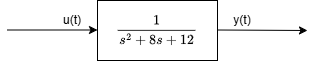
\includegraphics[width=\linewidth]{fig/systempods.drawio.png}
\end{center}
\subsubsection*{Odpowiedź impulsowa \{k(t)\}}
\begin{equation*}
    k(t) = \delta (t) \Rightarrow U(s) = \mathcal{L}\{\delta(t)\}=1
\end{equation*}
\begin{equation*}
    Y(s) = \frac{1}{s^2 + 8s +12}  \quad \Bigg| \ \mathcal{L}^{-1}\{\}
\end{equation*}
\begin{equation*}
    Y(s) = \frac{1}{(s+6)(s+2)} = \frac{A}{s+6} + \frac{B}{s+2} =
\end{equation*}
\begin{equation*}
    = -\frac{1}{4}\frac{1}{s+6} + \frac{1}{4}\frac{1}{s+2} \quad \Bigg| \ \mathcal{L}^{-1}\{\} 
\end{equation*}
\begin{equation}
    k(t) = -\frac{1}{4}(\mathrm{e}^{-6t} - \mathrm{e}^{-2t})
\end{equation}
\subsubsection*{Odpowiedź skokowa \{$\lambda(t)$\}}
\begin{equation*}
    \lambda(t) = 1(t) => U(s) = \mathcal{L}\{1(t)\} = \frac{1}{s}
\end{equation*}
\begin{equation*}
    Y(s) = \frac{1}{s(s+6)(s+2)} = \frac{A}{s} + \frac{B}{s+6} + \frac{C}{s+2}=
\end{equation*}
\begin{equation*}
   = \frac{1}{12}\frac{1}{s} + \frac{1}{24}\frac{1}{s+6} - \frac{1}{8}\frac{1}{s+2}  \quad \Bigg| \ \mathcal{L}^{-1}\{\}
\end{equation*}
\begin{equation}
    \lambda(t) = \frac{1}{12} + \frac{1}{24}\mathrm{e}^{-6t} -\frac{1}{8}\mathrm{e}^{-2t}
\end{equation}

\subsection{Symulacja komputerowa}
Równanie zapisano w~postaci równań stanu ($x_1=y,\ x_2=\dot y$):
\begin{equation}
    \dot{x} = \underbrace{\begin{bmatrix} 0 & 1 \\ -12 & -8 \end{bmatrix}}_{A}x
            + \begin{bmatrix} 0 \\ 1 \end{bmatrix}u, \quad
    y = \begin{bmatrix} 1 & 0 \end{bmatrix}x,
	\end{equation}
Odpowiedzi impulsową i skokową wyznaczono dodatkowo funkcjami \texttt{impulse}
i \texttt{step}.

\begin{center}
    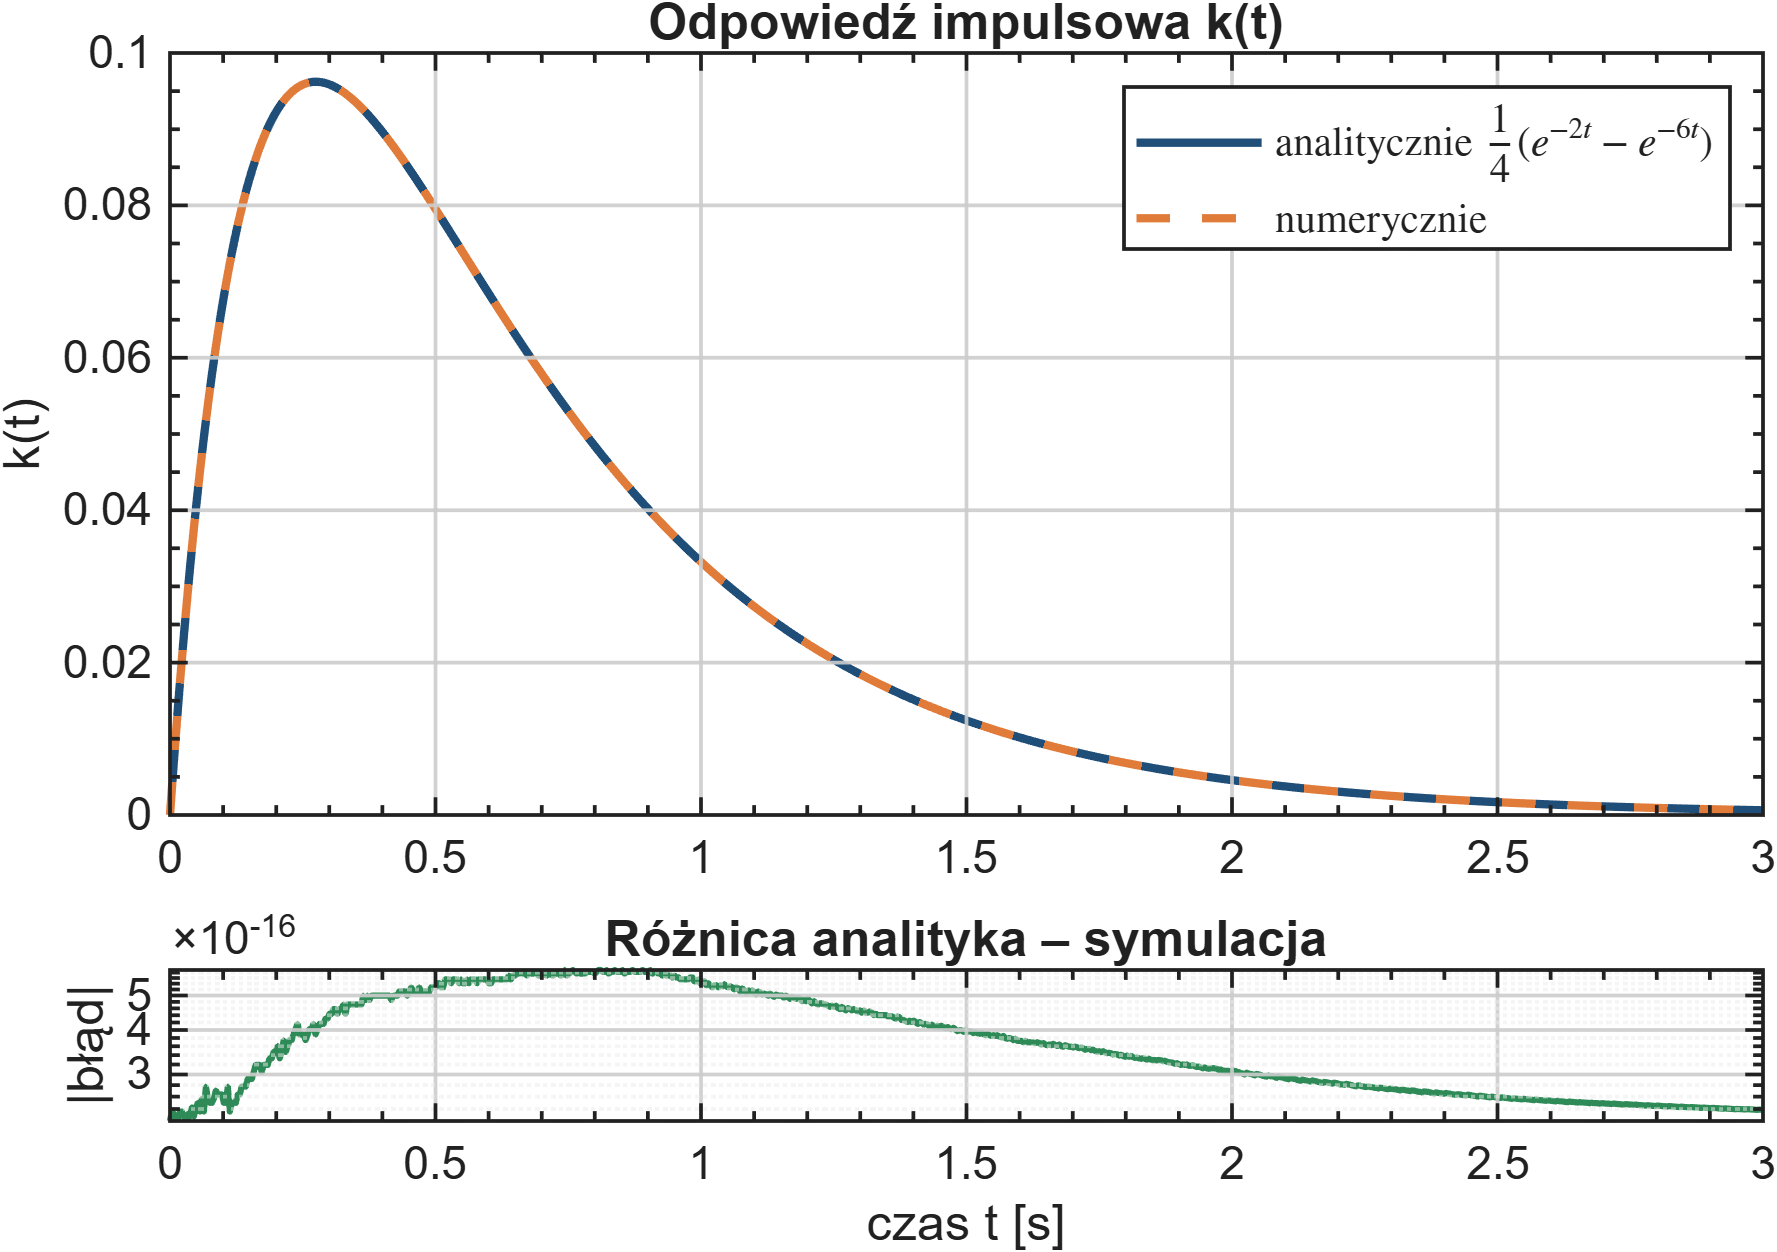
\includegraphics[width=\linewidth]{fig/odpowiedz_impulsowa.png}
    \captionof{figure}{Odpowiedź impulsowa $k(t)$: porównanie wyniku analitycznego
    z symulacją oraz wartość błędu bezwzględnego (skala logarytmiczna).}
    \label{fig:p1imp}
\end{center}

\begin{center}
    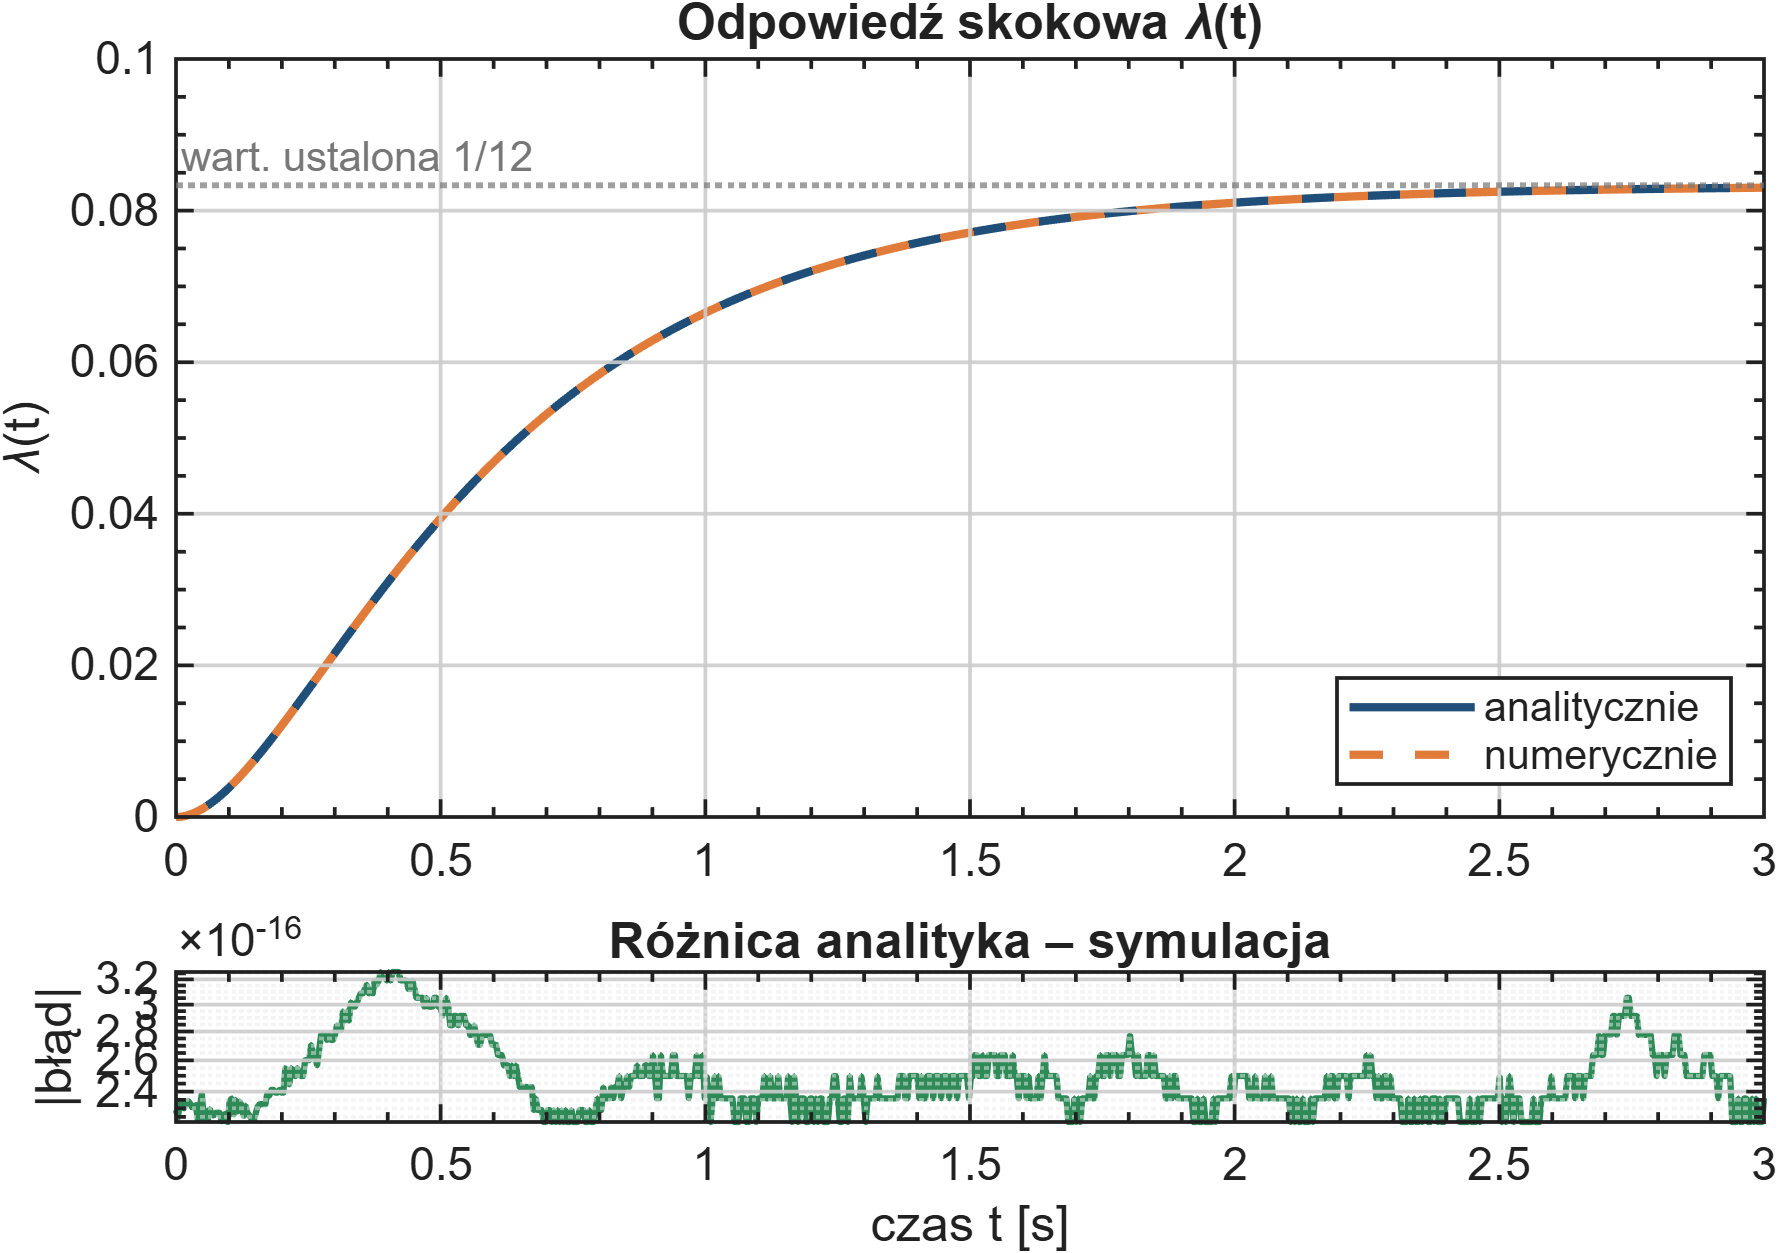
\includegraphics[width=\linewidth]{fig/odpowiedz_skokowa.png}
    \captionof{figure}{Odpowiedź skokowa $\lambda(t)$ wraz z wartością ustaloną
    $1/12$ oraz błędem względem rozwiązania analitycznego.}
    \label{fig:p1step}
\end{center}

\subsection{Porównanie wyników i wnioski (cz. 1)}
Krzywe analityczne i~numeryczne pokrywają się w granicach dokładności.
Maksymalny błąd bezwzględny odpowiedzi impulsowej wyniósł $\sim\!4\cdot10^{-16}$,
a skokowej $\sim\!1\cdot10^{-16}$. Potwierdza to
poprawność zarówno wyprowadzeń analitycznych, jak i modelu numerycznego. 


\section{Analiza częstotliwościowa}

\subsection{Charakterystyka analityczna}
Podstawiając $s=j\omega$ do transmitancji:
\begin{equation}
    K(j\omega) = \frac{1}{(12-\omega^2) + j\,8\omega}.
\end{equation}
Moduł i~argument (charakterystyka amplitudowo-fazowa):
\begin{align}
    |K(j\omega)| &= \frac{1}{\sqrt{(12-\omega^2)^2 + (8\omega)^2}},\\[2pt]
    \varphi(\omega) &= -\arctan\!\frac{8\omega}{12-\omega^2}.
\end{align}
Wartości graniczne: $|K(0)|=\tfrac{1}{12}$ ($\varphi=0$), a dla $\omega\to\infty$
moduł maleje jak $\omega^{-2}$, zaś $\varphi\to-180^\circ$.
Dla $\omega=\sqrt{12}=\omega_n$ część rzeczywista mianownika zeruje się, więc
$\varphi=-90^\circ$.

\subsection{Wyznaczenie eksperymentalne}
Układ pobudzano sygnałem $u(t)=\sin(\omega_0 t)$ dla zestawu pulsacji $\omega_0$.

\begin{center}
\captionof{table}{Punkty charakterystyki Nyquista wyznaczone z odpowiedzi ustalonej}
\label{tab:nyquist}
\begin{tabular}{|c|r|r|r|r|}
\hline
$\omega$ [rad/s] & $\mathrm{Re}\{G\}$ & $\mathrm{Im}\{G\}$ & $|G|$ & $\varphi$ [$^\circ$] \\
\hline
0.50 & $ 0.076$ & $-0.026$ & $0.081$ & $ -18.8$ \\
1.00 & $ 0.059$ & $-0.043$ & $0.074$ & $ -36.0$ \\
2.00 & $ 0.025$ & $-0.050$ & $0.056$ & $ -63.4$ \\
3.00 & $ 0.005$ & $-0.041$ & $0.041$ & $ -82.9$ \\
4.00 & $-0.004$ & $-0.031$ & $0.031$ & $ -97.1$ \\
6.00 & $-0.008$ & $-0.017$ & $0.019$ & $-116.6$ \\
9.00 & $-0.007$ & $-0.007$ & $0.010$ & $-133.8$ \\
\hline
\end{tabular}
\end{center}

Po zaniku składowej przejściowej rejestrowano odpowiedź ustaloną
$y_\text{ust}(t)=A\sin(\omega_0 t+\varphi)$. Amplitudę $A$ i~fazę $\varphi$ wyznaczano
metodą najmniejszych kwadratów

\begin{center}
    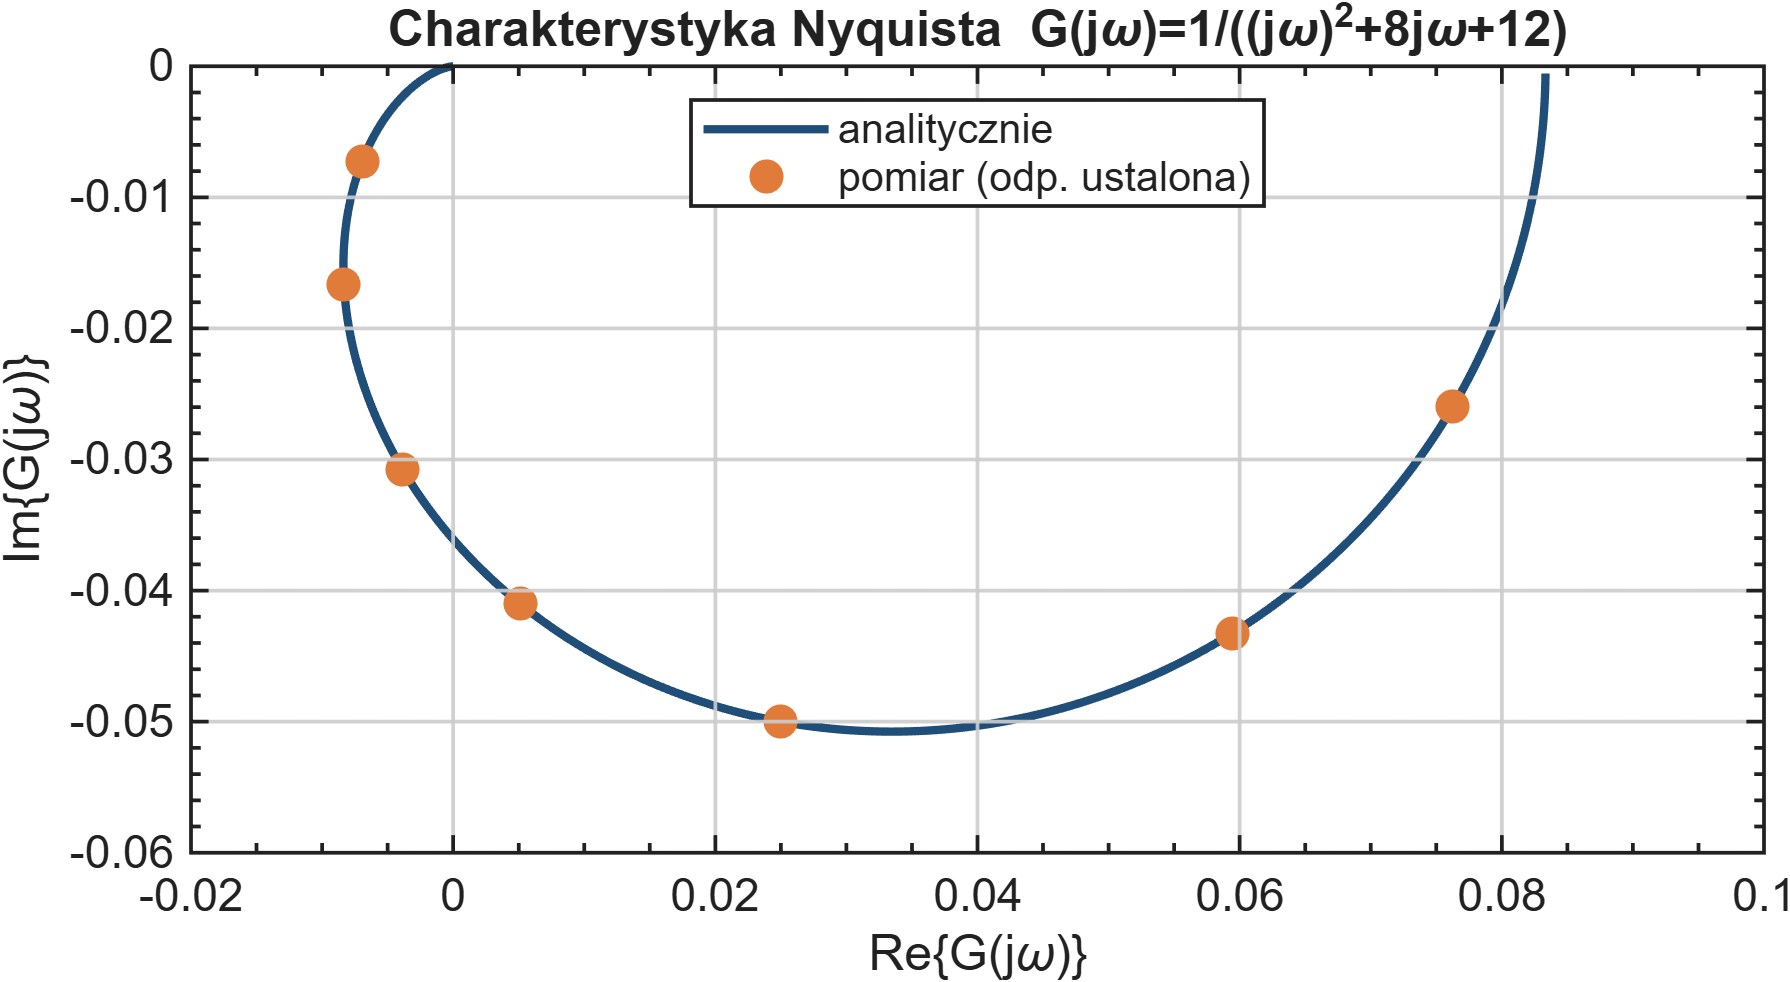
\includegraphics[width=0.92\linewidth]{fig/nyquist.png}
    \captionof{figure}{Charakterystyka Nyquista $K(j\omega)$}
    \label{fig:nyq}
\end{center}

\subsection{Wnioski (cz. 2)}
Charakterystyki wyznaczone analitycznie i~eksperymentalnie są praktycznie identyczne
(różnice $<\!0{,}1\%$ amplitudy oraz $<\!0{,}1^\circ$ fazy). Układ ma charakter \textbf{dolnoprzepustowy}:
najsilniej przenosi składowe wolnozmienne, a~powyżej $\omega_n$ tłumi sygnał. Charakterystyka Nyquista nie obejmuje punktu $(-1,j0)$, co zapowiada
stabilność układu zamkniętego dla szerokiego zakresu wzmocnień

\section{Stabilność systemu}
\subsection{Kryterium Hurwitza}
Aby system był stabilny w kryterium hurwitza to minory główne wiodące macierzy Hurwitza zbudowanej ze współczynników mianownika transmitancji systemu muszą być dodatnia.
	\begin{gather*} 
	\begin{bmatrix}
		8 & 0\\
		1 & 12
	\end{bmatrix}\\
	\Delta_1 = 8 >0\\
	\Delta_2 = 8 \cdot 12-1 \cdot 0=96>0\\
	\Delta_1 > 0 \land \Delta_2 > 0 \implies \textbf{system\ stabilny}
	\end{gather*} 
\subsection{Kryterium Michajłowa}
Aby system był stabilny w kryterium Michajłowa 
\begin{equation*}
	\forall_{\omega \in [0, \infty)} M(j\omega) \neq 0
\end{equation*}
oraz
\begin{equation*}
	\Delta arg_{0\ge \omega \ge \infty} M(j\omega)=m\frac{\pi}{2}
\end{equation*} 
Z wykresu \ref{fig:michajlow} można odczytać że zarówno pierwszy warunek tj. nie przechodzenie przez punkt (0,0) jak i drugi tj. przejście przez 2 ćwiartki układu współrzędnych są spełnione a więc na mocy kryterium Michajłowa system jest stabilny.
\begin{center}
	\centering
	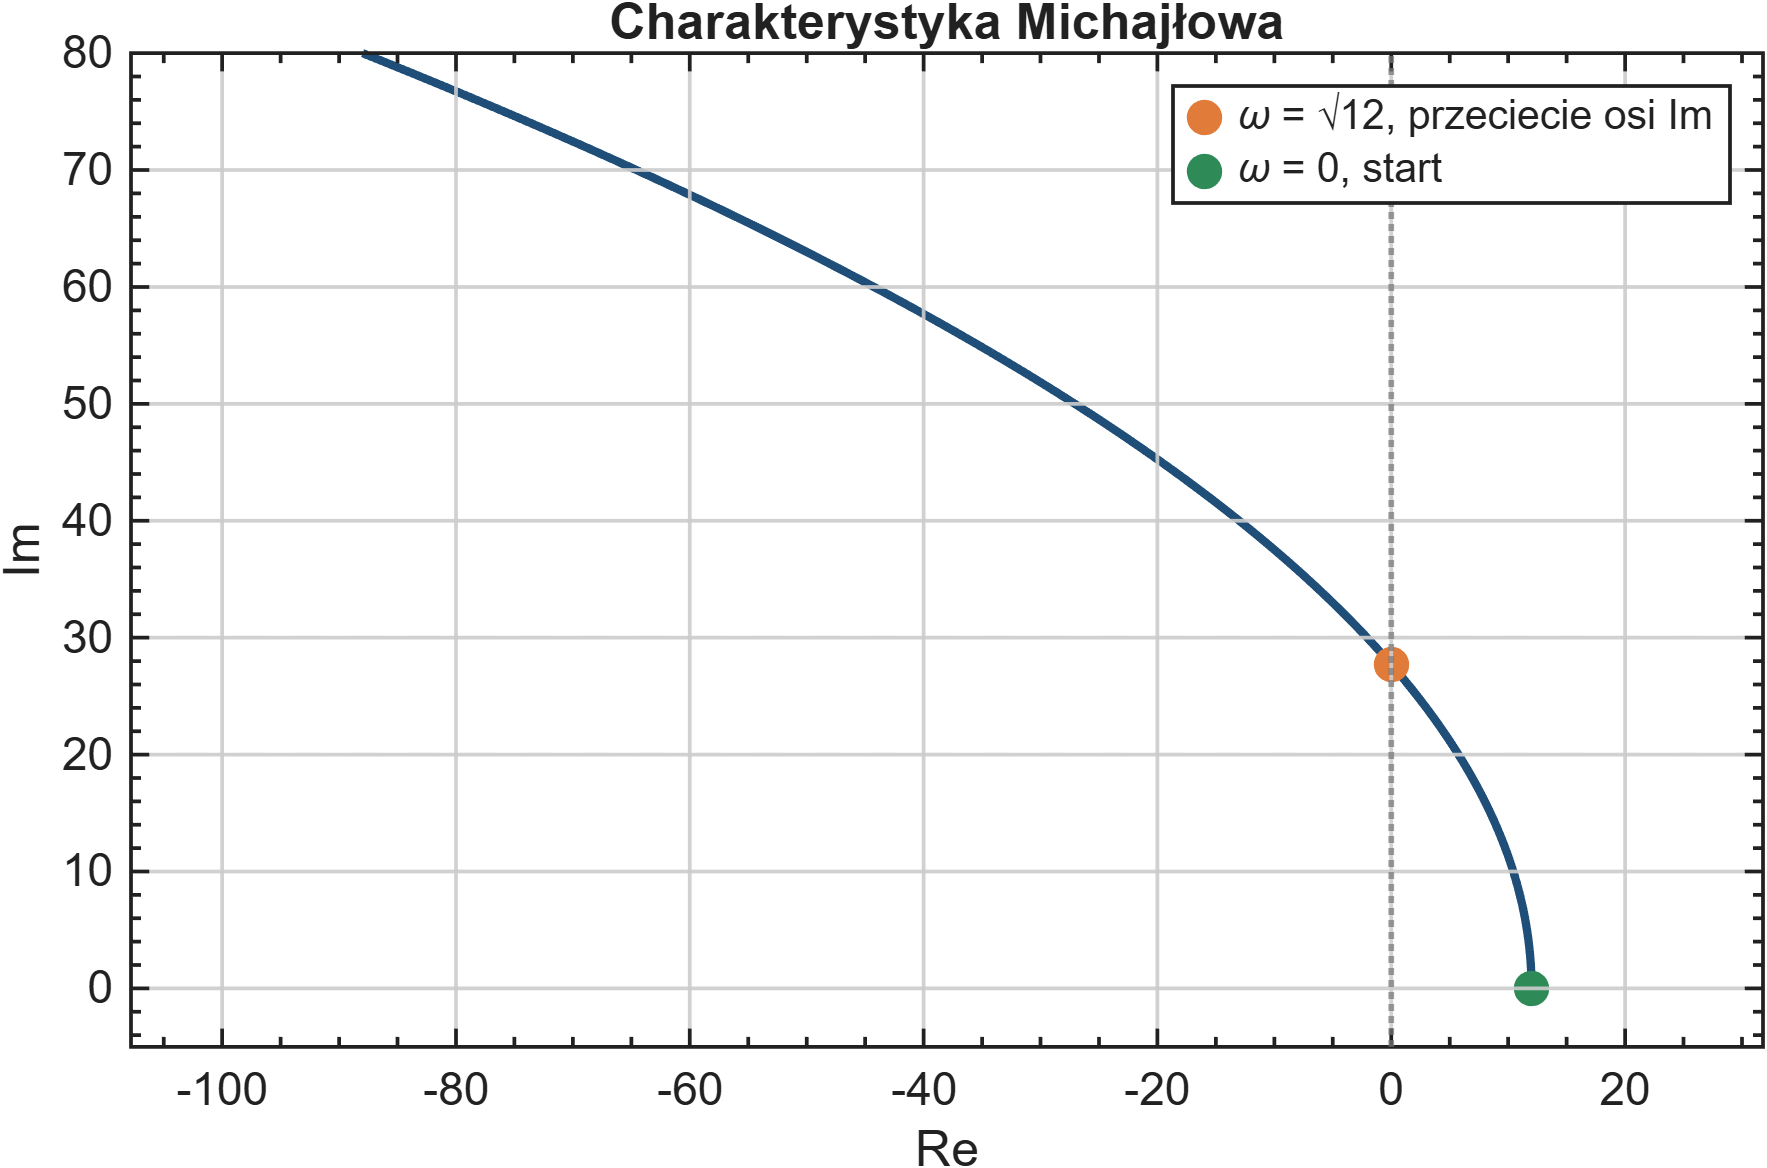
\includegraphics[width=0.92\linewidth]{fig/michajlow.png}
	\captionof{figure}{Charakterystyka Michajłowa}
	\label{fig:michajlow}
\end{center}

\subsection{Stabilność układu zamkniętego z regulatorem P}

Zbadano układ w ujemnej pętli z regulatorem typu P. Wybrano trzy wzmocnienia $k \in \textbf{\{-15, -12, -5\}}$ zapewniające odpowiednio niestabilności, granicę stabilności oraz stabilność. Odpowiedzi impulsowe przedstawiono na rys. \ref{fig:unstable}, \ref{fig:granica} i \ref{fig:stable}. W przypadku gdy system jest stabilny odpowiedź impulsowa zanika do 0, gdy system jest na granicy stabilności przyjmuje wartość $\neq 0$ oraz $< \infty$, a gdy jest niestabilny dąży do $\infty$.
\begin{center}\small
\begin{tabularx}{\linewidth}{l l l}
\toprule
$k_p$ & bieguny & charakter \\
\midrule
$-15$    & $-8.36;\ +0.36$  & niestabilny \\
$-12$ & $0;\ -8$ & granica \\
$-5$   & $-7;\ -1$  & stabilny \\
\bottomrule
\end{tabularx}
\end{center}

\begin{center}
	\centering
	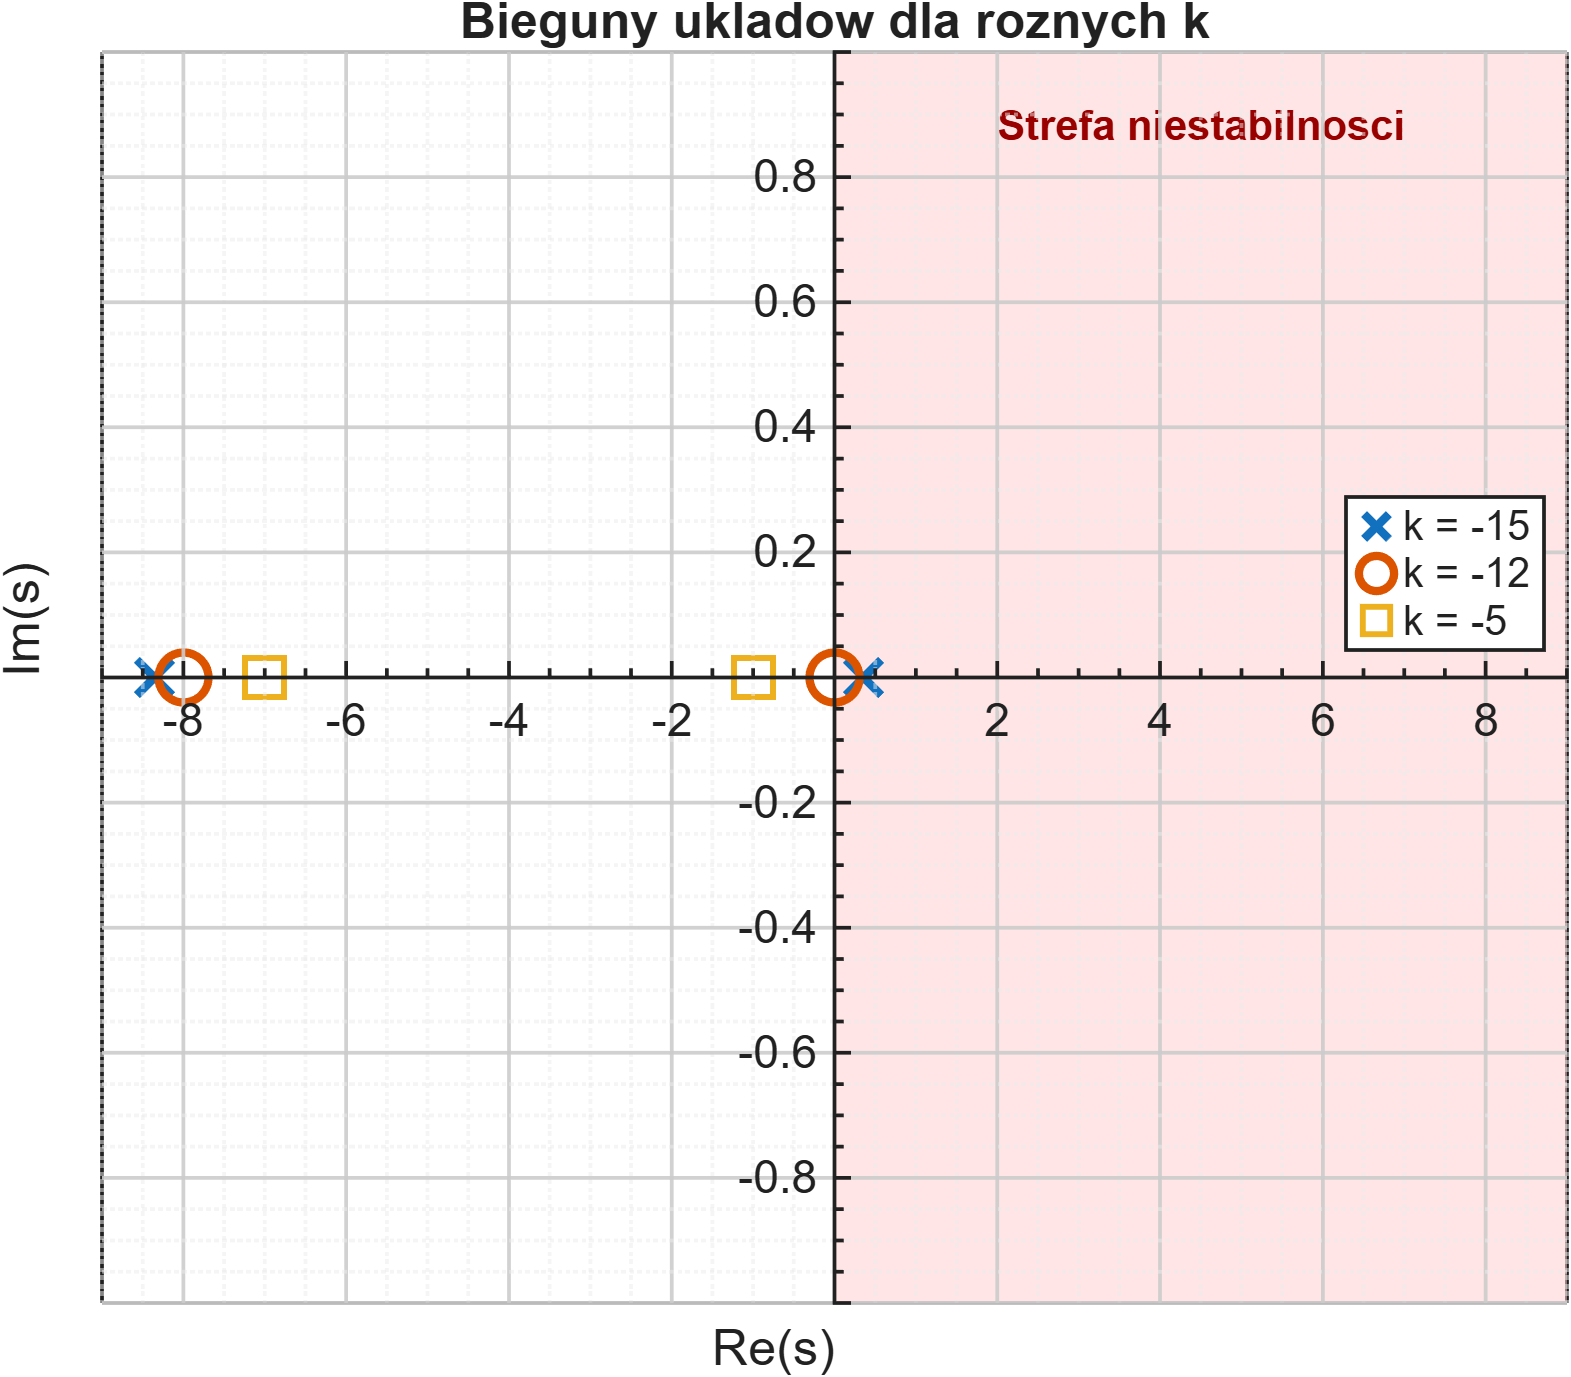
\includegraphics[width=0.92\linewidth]{fig/bieguny.png}
\end{center}
\begin{center}
	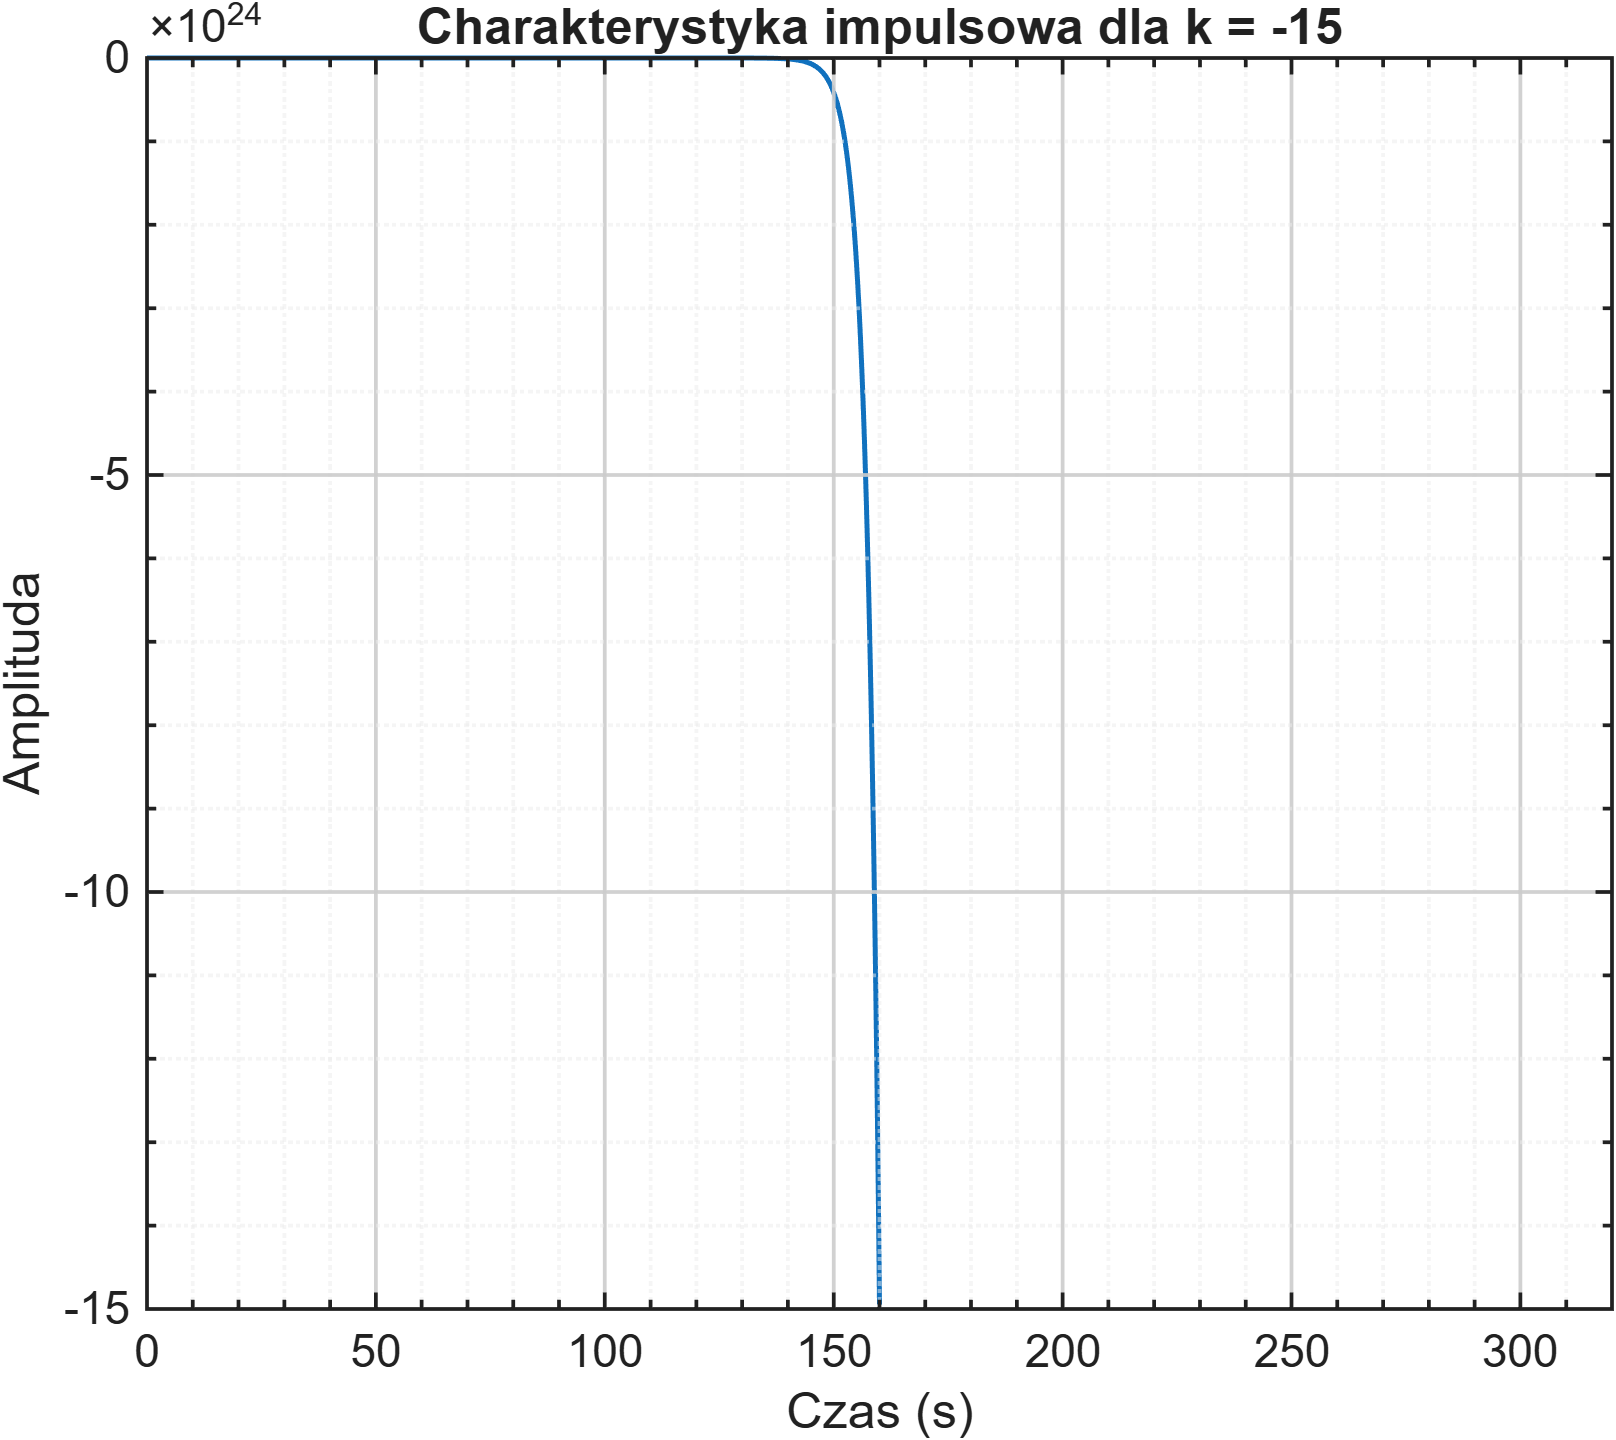
\includegraphics[width=0.92\linewidth]{fig/k=-15.png}
	\captionof{figure}{Charakterystyka impulsowa dla k = -15}
	\label{fig:unstable}
\end{center}
\begin{center}
	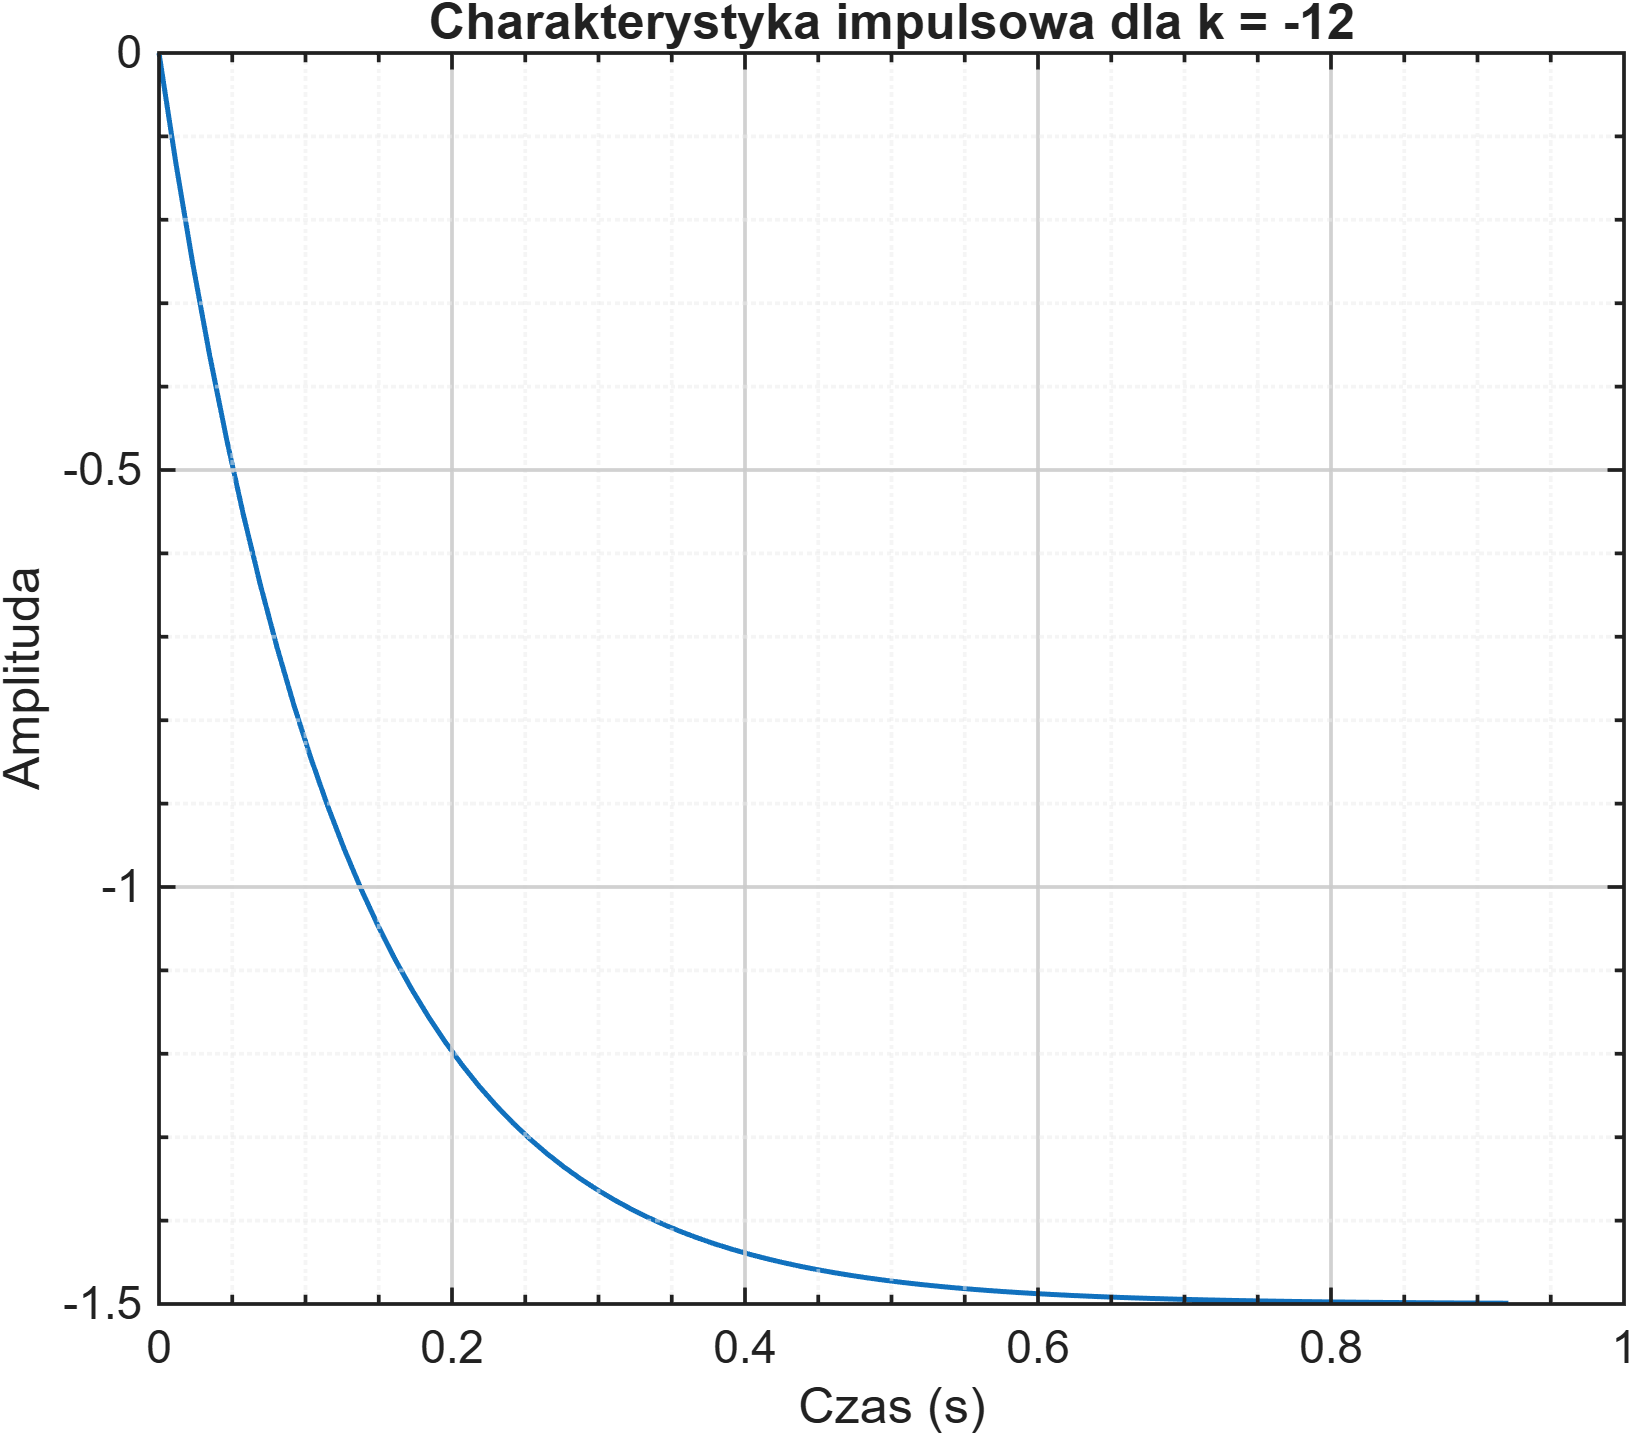
\includegraphics[width=0.92\linewidth]{fig/k=-12.png}
	\captionof{figure}{Charakterystyka impulsowa dla k = -12}
	\label{fig:granica}
\end{center}
\begin{center}
	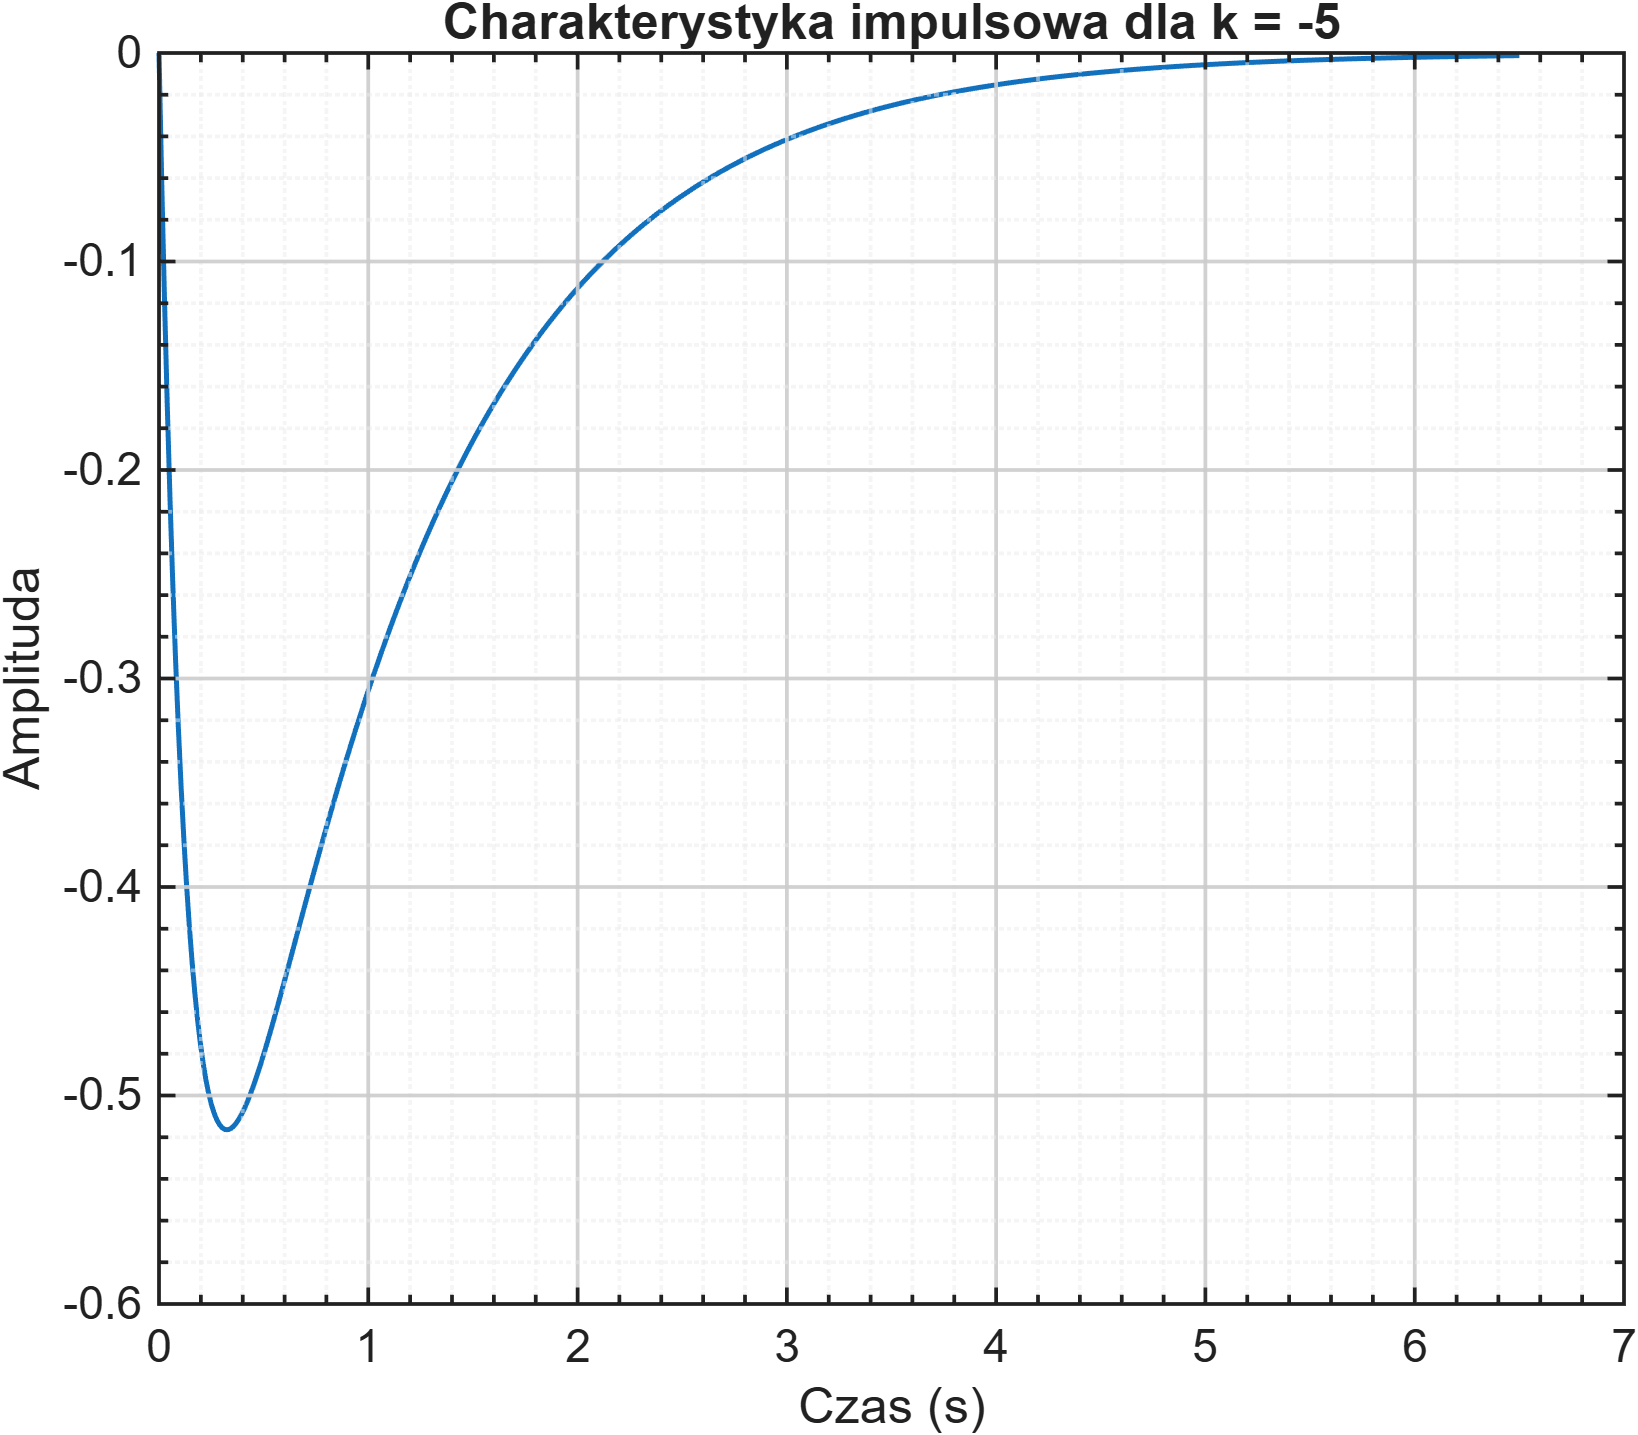
\includegraphics[width=0.92\linewidth]{fig/k=-5.png}
	\captionof{figure}{Charakterystyka impulsowa dla k = -5}
	\label{fig:stable}
\end{center}

\subsection{Porównanie kryteriów i wnioski (cz. 3)}
Trzy zastosowane metody dają spójny obraz stabilności:
\begin{itemize}[leftmargin=*, nosep]
\item \textbf{Hurwitz} kryterium algebraiczne, najszybsze; bezpośrednio podaje
warunek $k_p>-12$, lecz nie informuje o~dynamice (rozkładzie biegunów).
\item \textbf{Michajłow} kryterium graficzne; potwierdza stabilność układu otwartego
poprzez analizę przyrostu argumentu, czytelne lecz wymagające wykreślenia hodografu.
\item \textbf{Analiza biegunów / pętli $k_p$} najbogatsza informacyjnie: pokazuje
nie tylko fakt stabilności, ale i~jej zapas oraz charakter odpowiedzi.
\end{itemize}


\section{Regulacja PID}
W kolejnych zadaniach transmitancja układu to: $K(s)=\frac{1}{s^4+5s^3+7s^2+8s+1}$
\subsection{Metoda Zieglera–Nicholsa}
Zgodnie z drugą metodą Zieglera-Nicholsa doprowadzono układ do niegasnących oscylacji i wyznaczono $K_u$ oraz $T_u$. Na ich podstawie wyznaczono wartości $K_p$, $T_i$ oraz $T_d$ na podstawie poniższej tabeli.\\
\begin{tabular}{|c|c|c|c|}
	\hline
	& $K_p$   & $T_i$    & $T_d$ \\ \hline
	P   & $0.5K_u $    & $\infty$ & 0     \\ \hline
	PI  & $0.45K_u $  & $0.54K_u/T_u $    & 0     \\ \hline
	PID & $0.6K_u $  & $1.2K_u/T_u $      & $0.075K_u/T_u $ \\ \hline
\end{tabular}\\
Odpowiedzi skokowe układu automatycznej regulacji przedstawiono na rys. \ref{fig:PZN}, \ref{fig:PIZN} oraz \ref{fig:PIDZN}.
\section{Dyskretyzacja systemu ciągłego}
Nastawy I dla poszczególnych T, T=.1 I= 4.6465,T=1 I= 32.1212, T=5 I=87.2727
\end{multicols*}
\begin{figure}
	\centering
	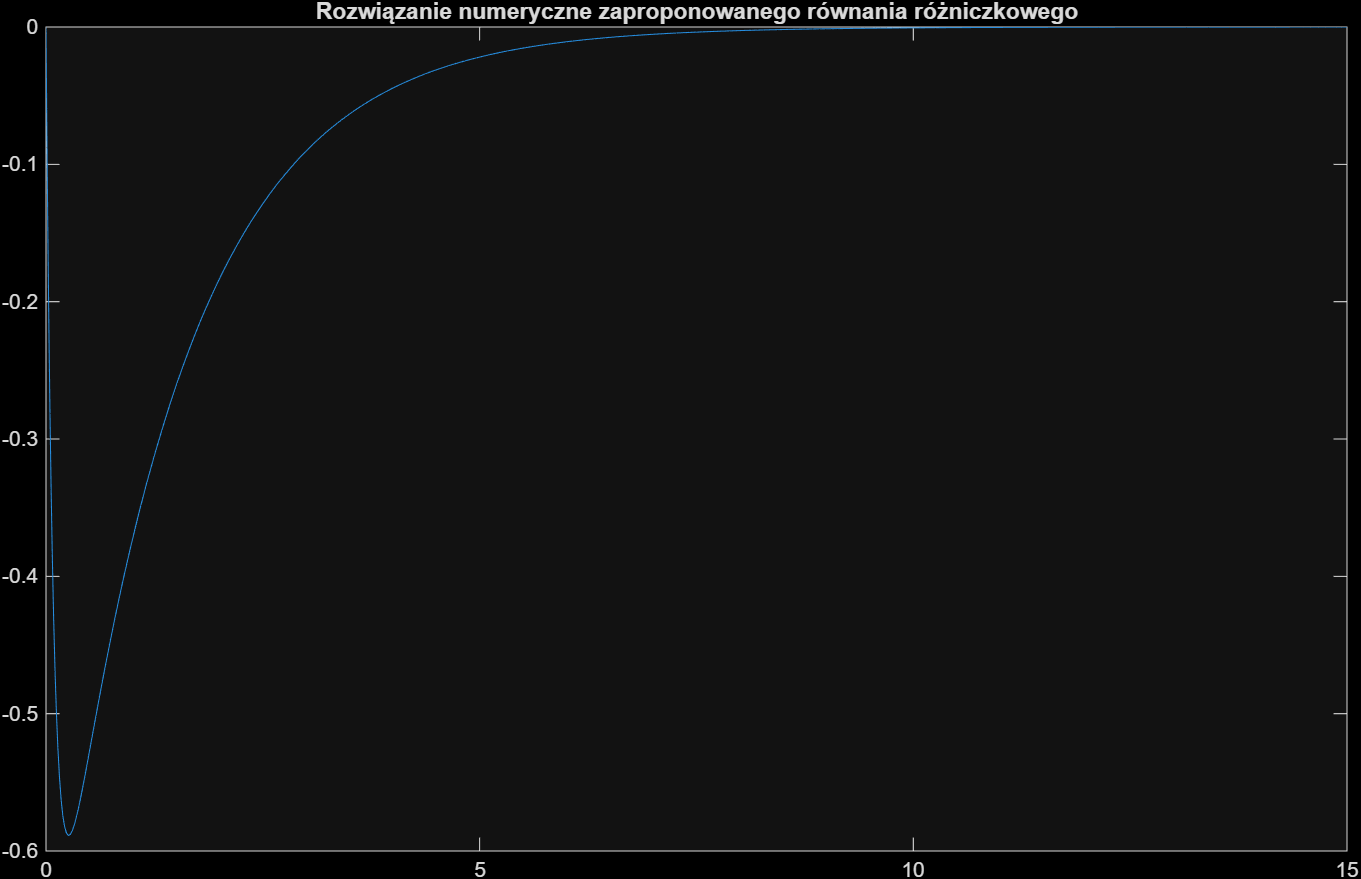
\includegraphics[width=0.7\linewidth]{../diff_equa}
	\caption[]{Numeryczne rozwiązanie równania}
	\label{fig:numrr}
\end{figure}

\begin{figure}
	\centering
	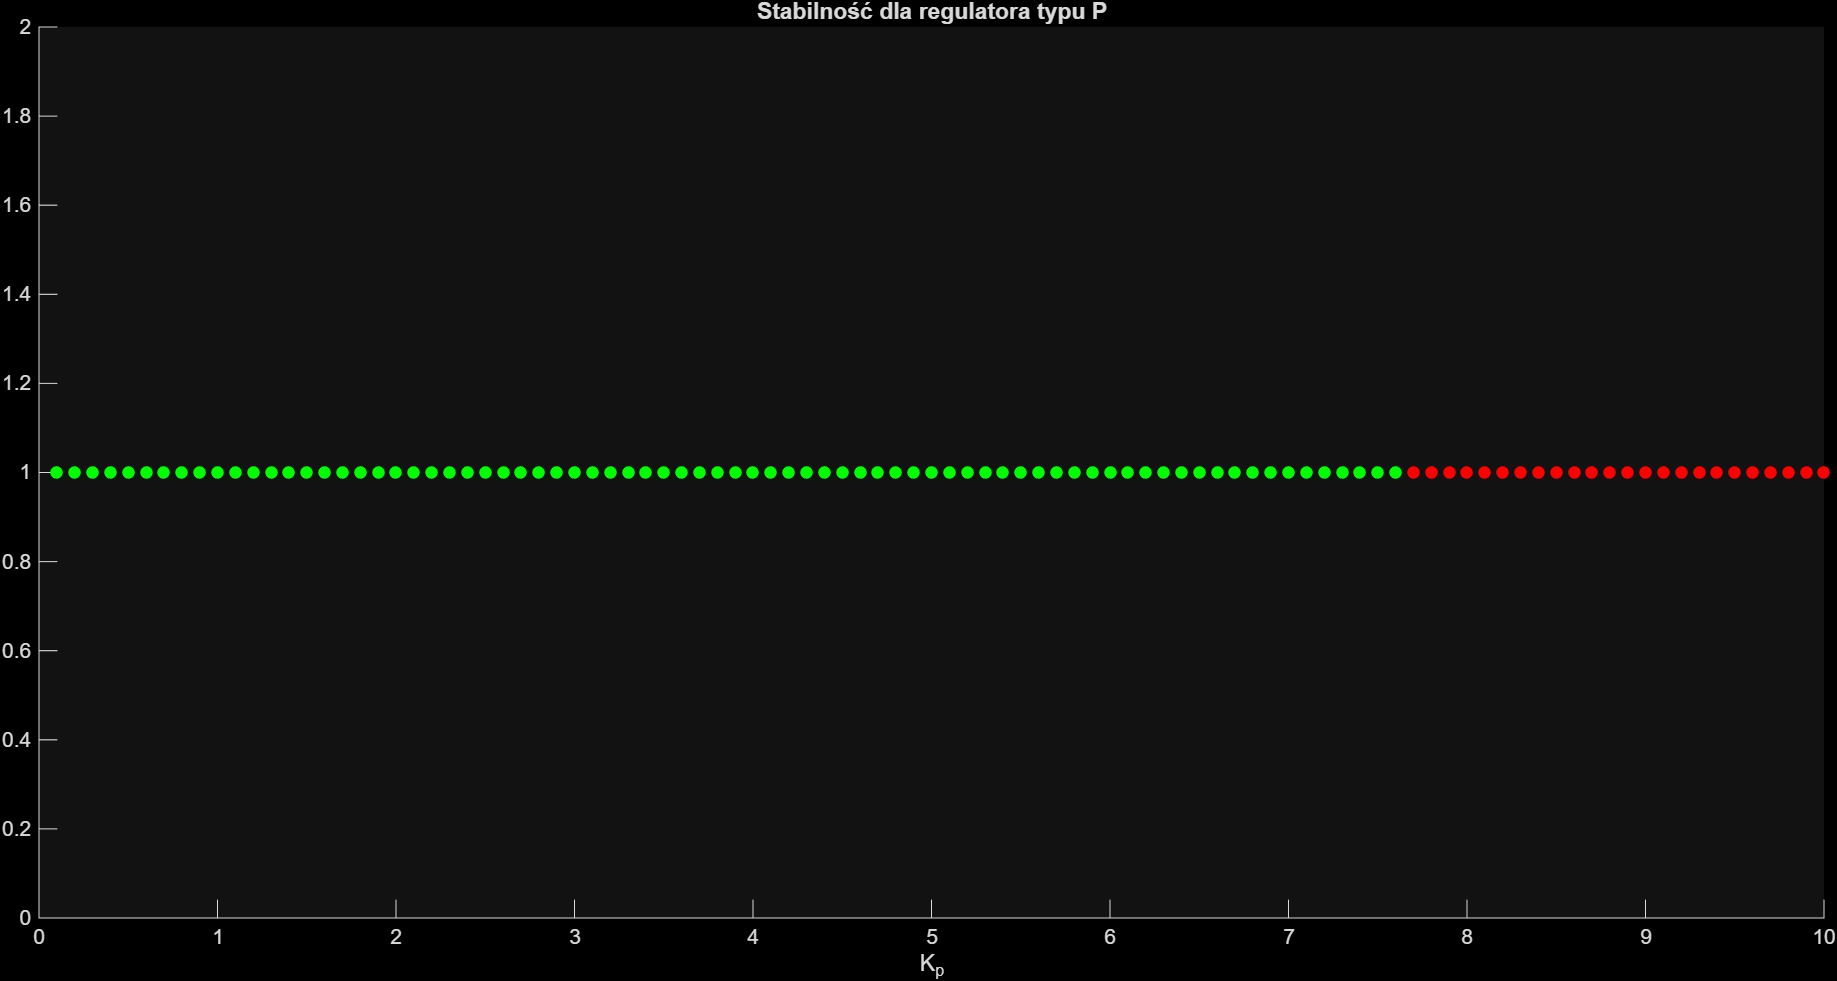
\includegraphics[width=0.7\linewidth]{../stabP}
	\caption{Wykres stabilności dla regulatora P}
	\label{fig:stabp}
\end{figure}
\begin{figure}
	\centering
	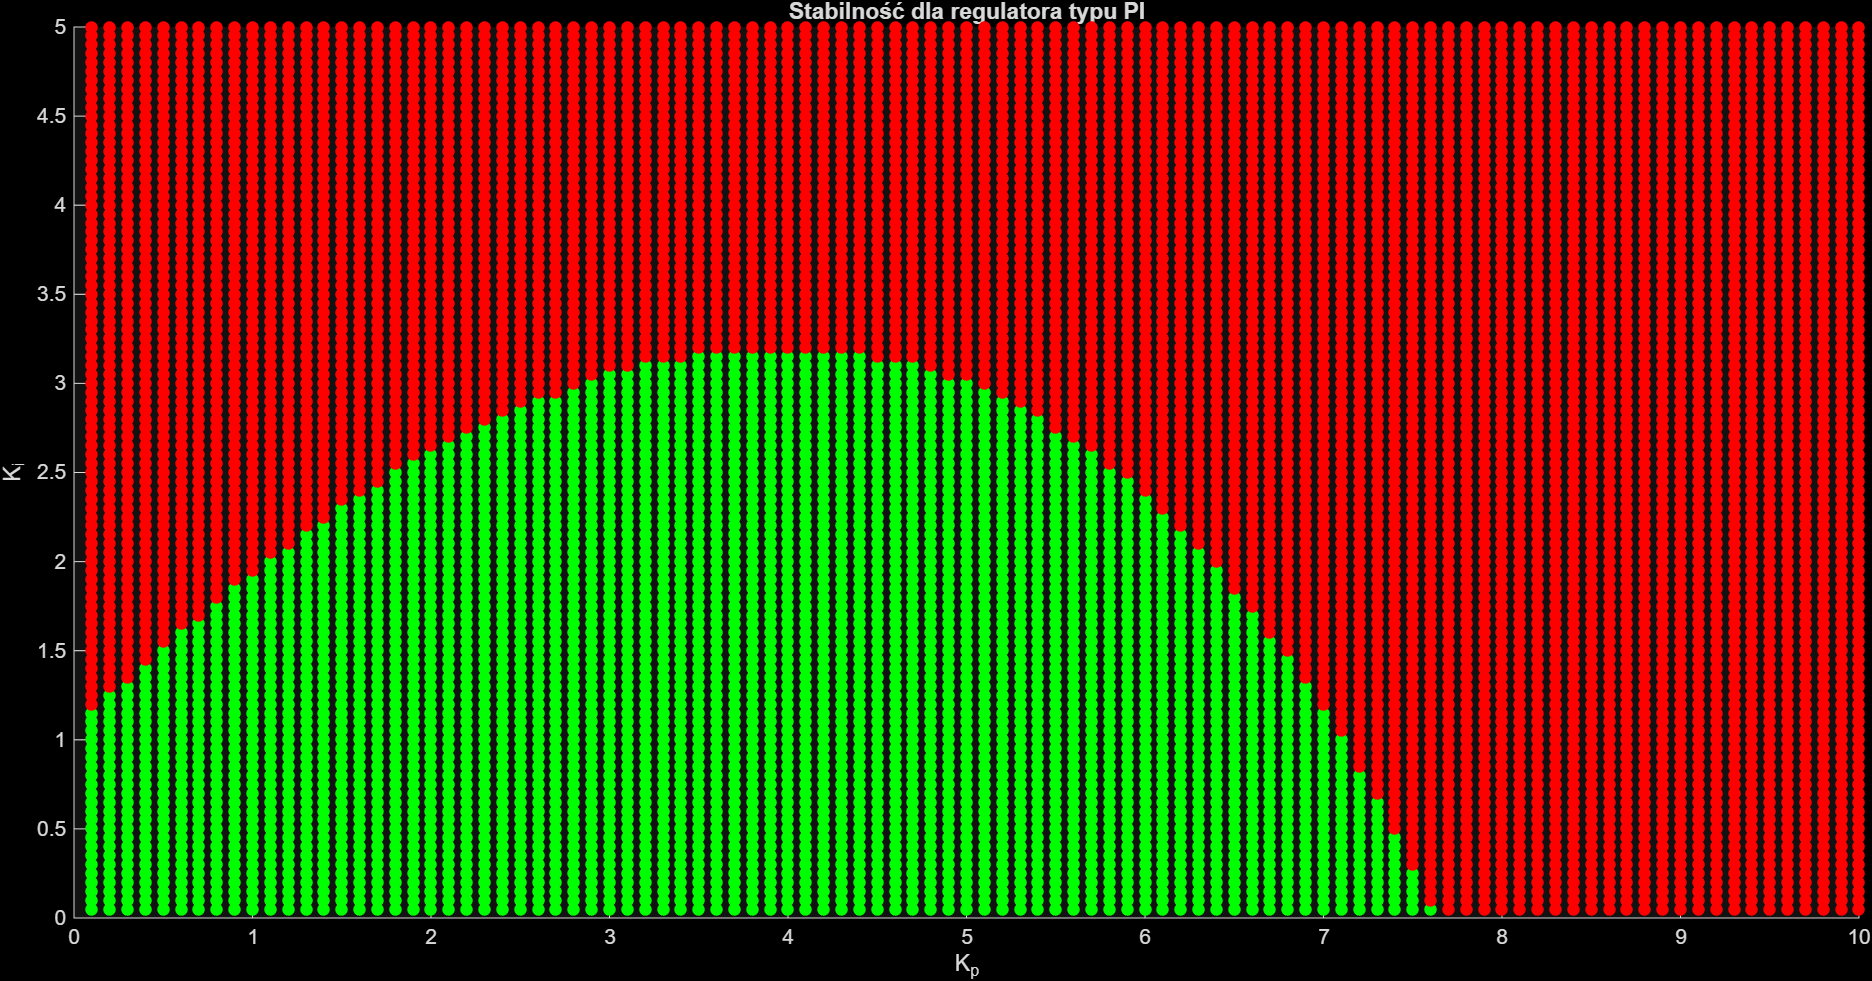
\includegraphics[width=0.7\linewidth]{../stabPI}
	\caption{Wykres stabilności dla regulatora PI}
	\label{fig:stabpi}
\end{figure}
\begin{figure}
	\centering
	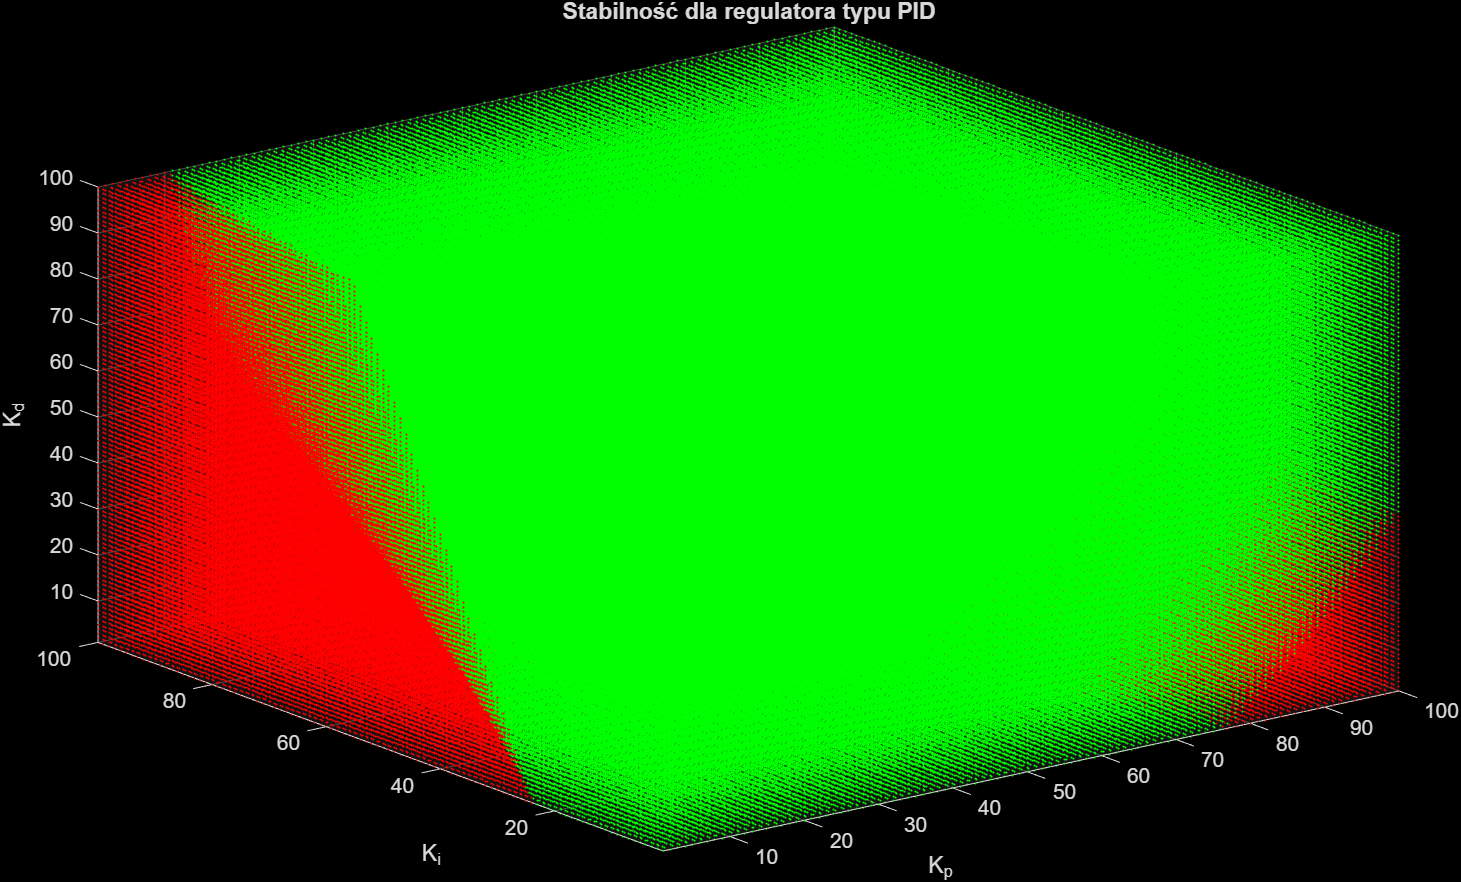
\includegraphics[width=0.7\linewidth]{../stabPID}
	\caption{Wykres stabilności dla regulatora PID}
	\label{fig:stabpid}
\end{figure}
\begin{figure}
	\centering
	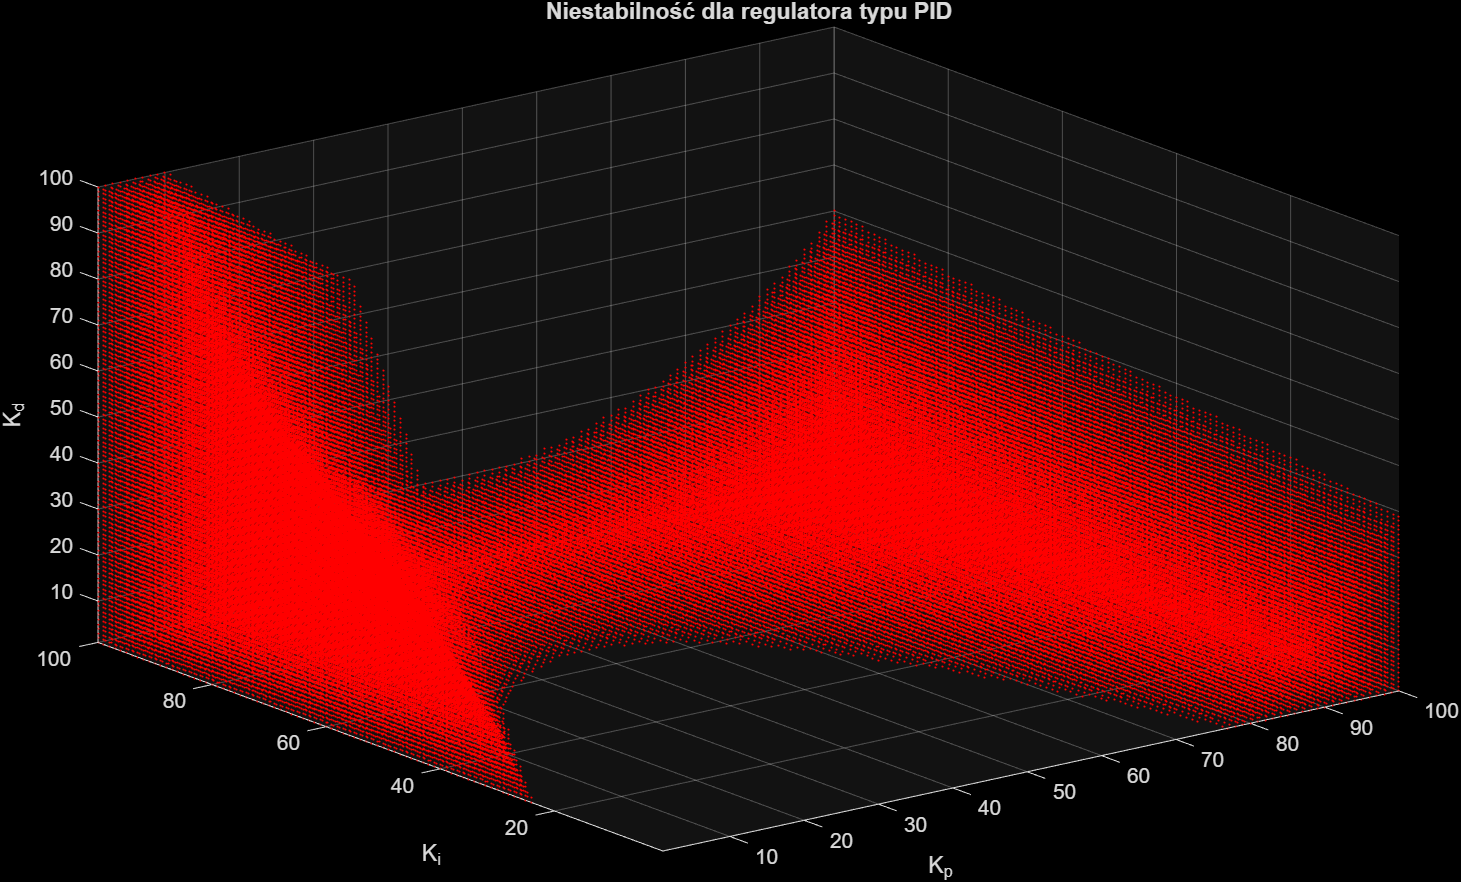
\includegraphics[width=0.7\linewidth]{../niestabPID}
	\caption{Wykres stabilności dla regulatora PID bez punktów oznaczających stabilność}
	\label{fig:niestabpid}
\end{figure}
\begin{figure}
	\centering
	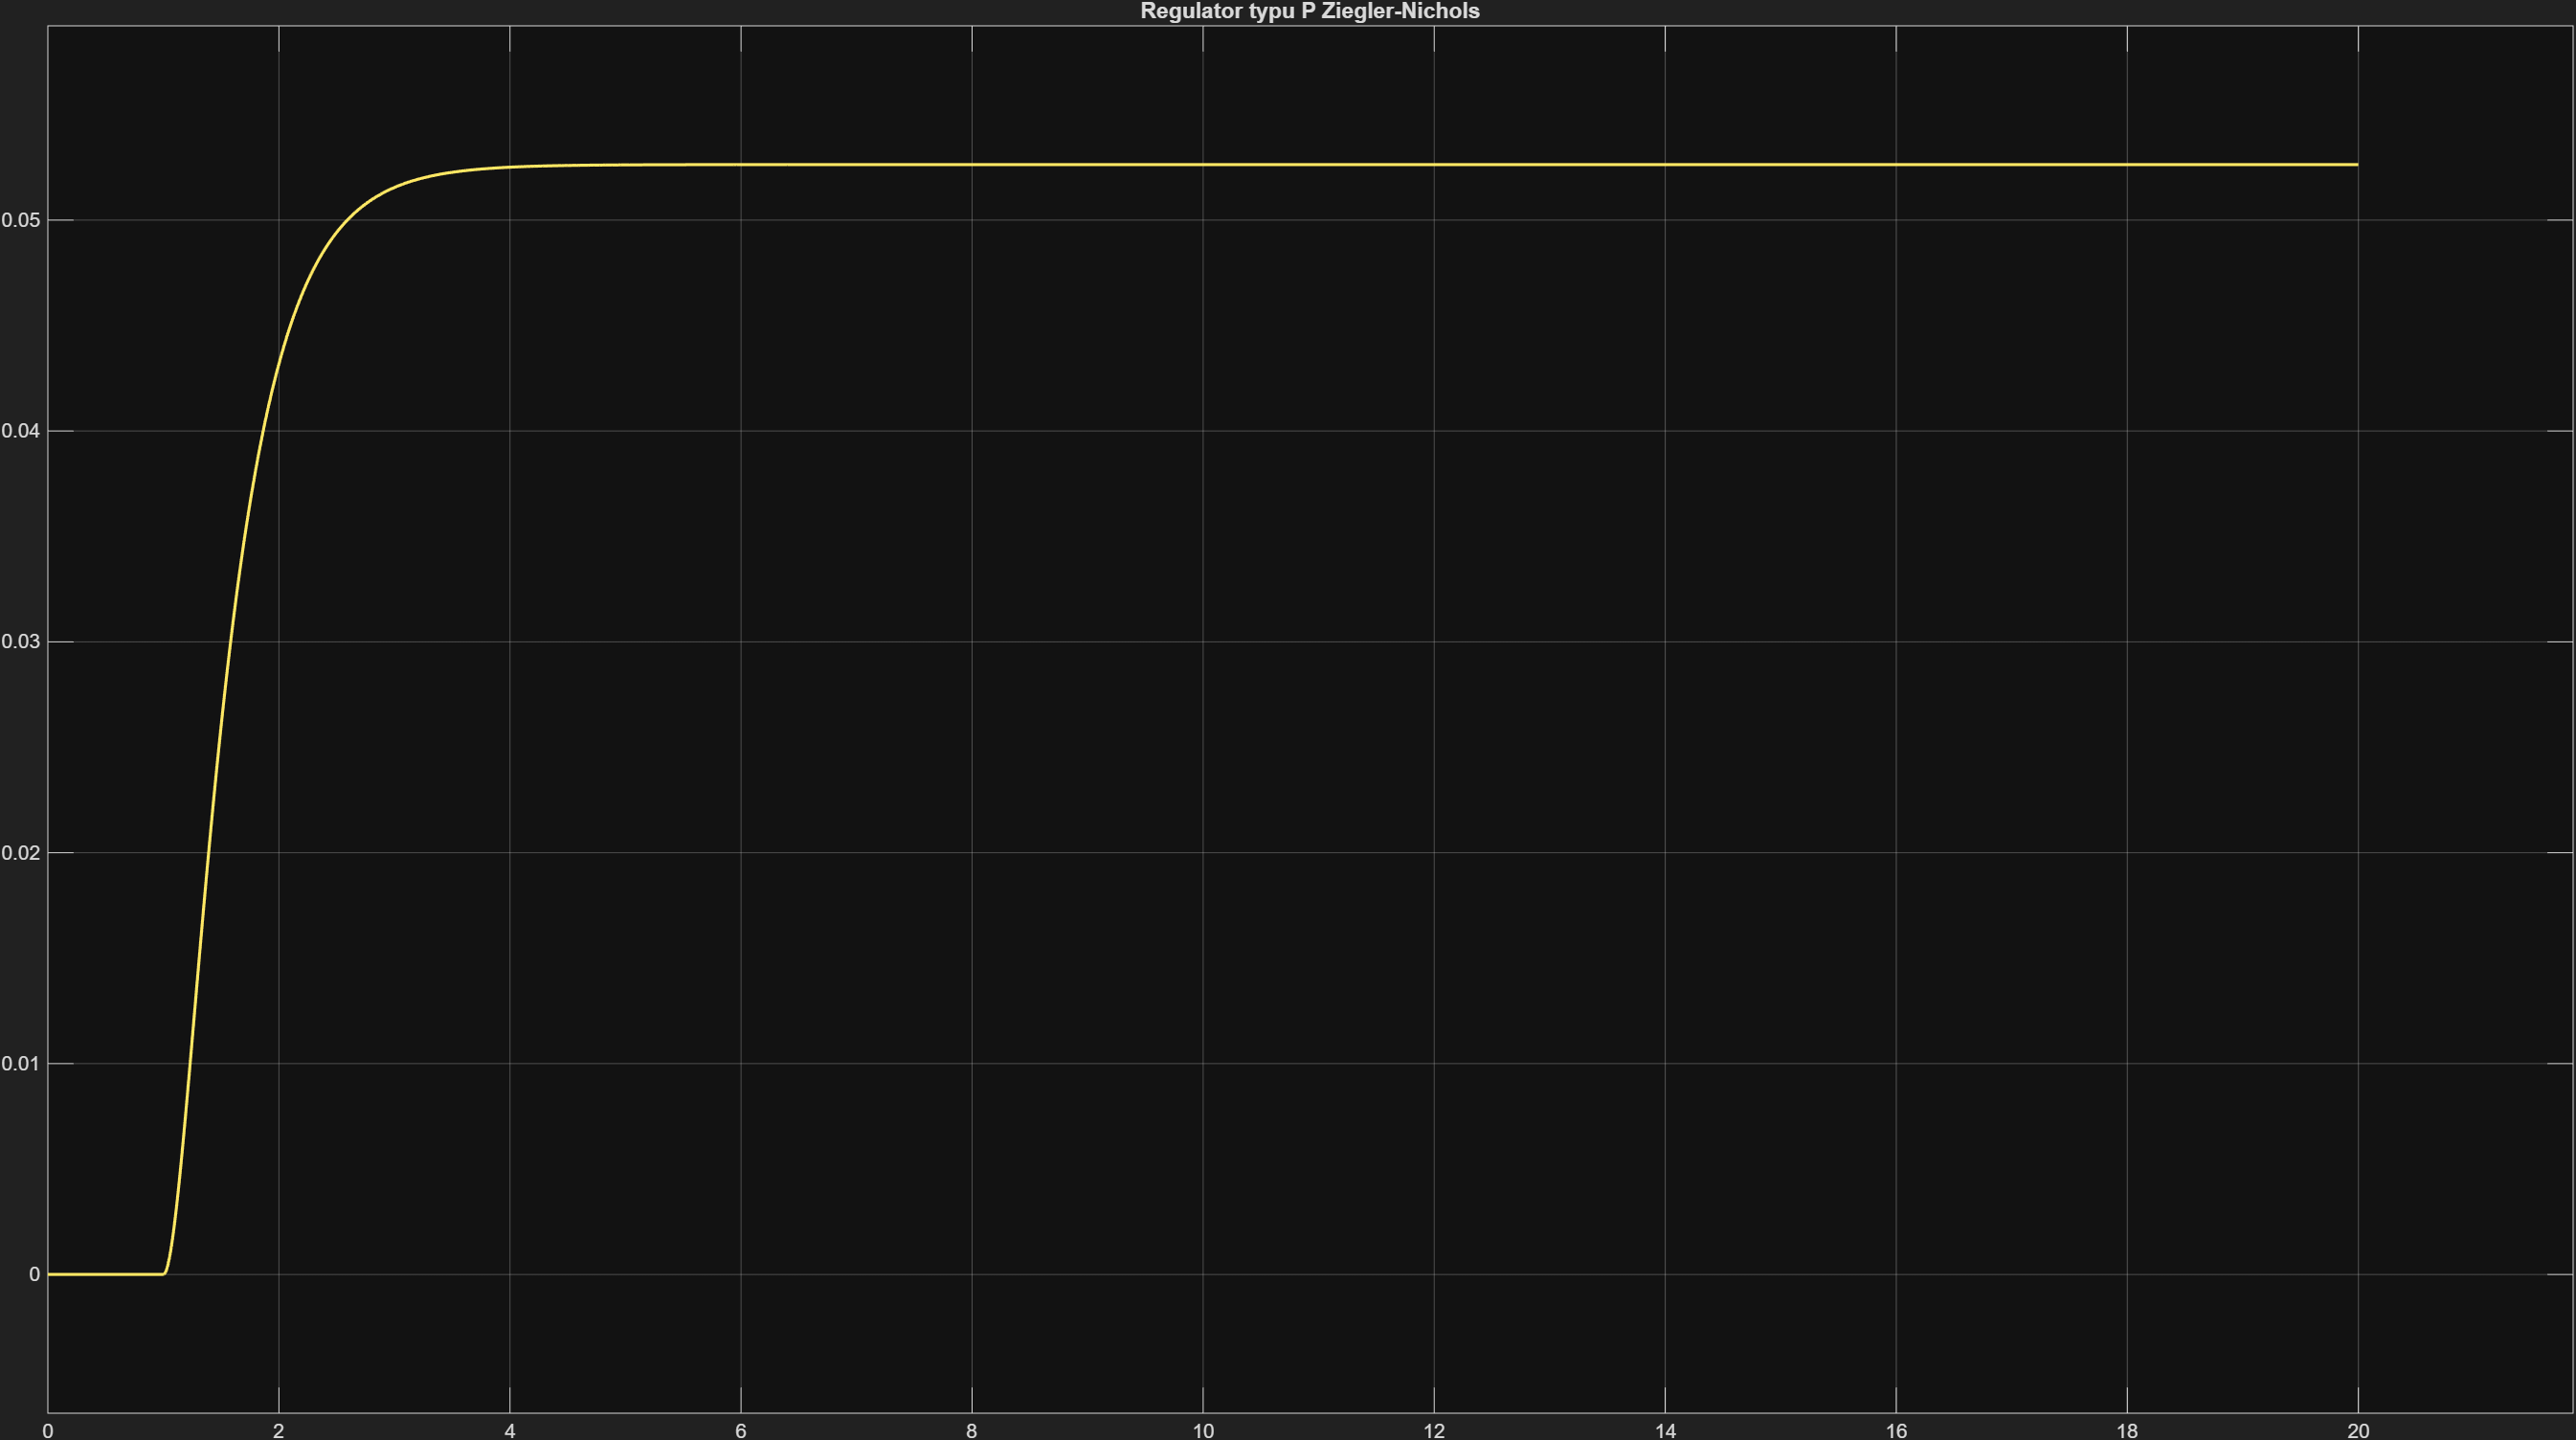
\includegraphics[width=0.7\linewidth]{../ScopePZN}
	\caption[]{Charakterystyka skokowa dla metody Zieglera-Nicholsa dla regulatora typu P}
	\label{fig:PZN}
\end{figure}
\begin{figure}
	\centering
	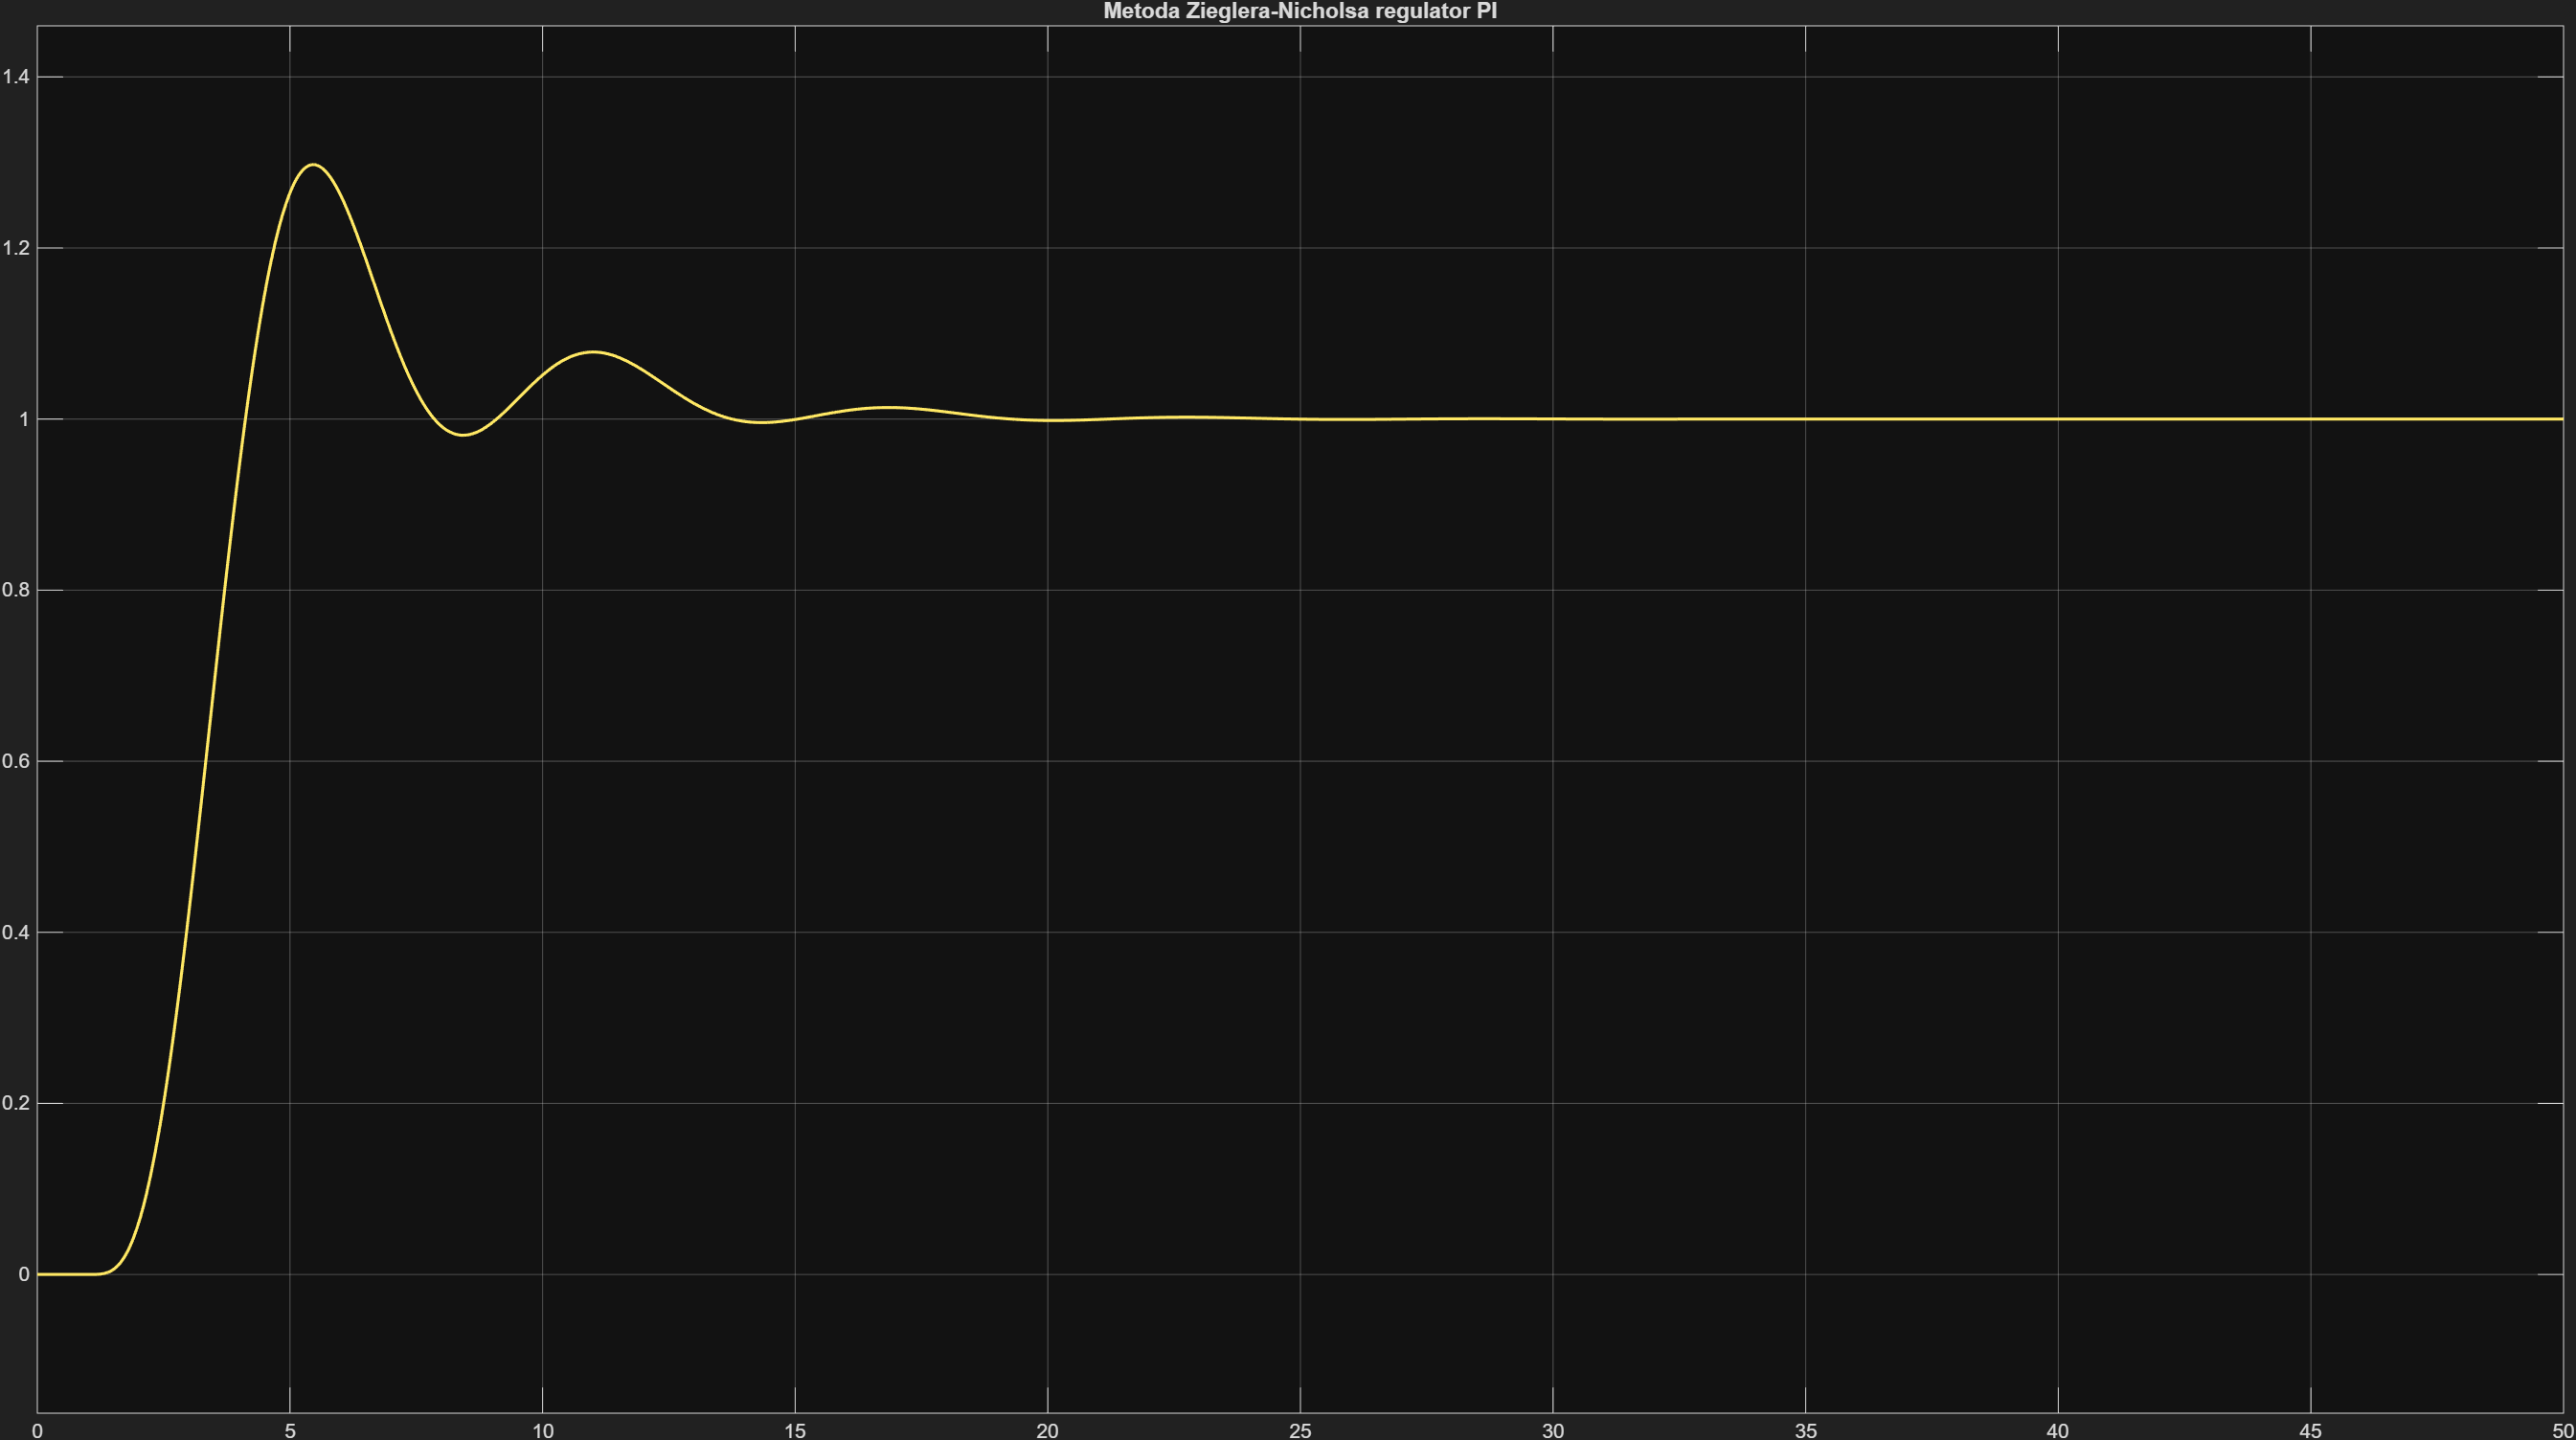
\includegraphics[width=0.7\linewidth]{../ScopePIZN}
	\caption[]{Charakterystyka skokowa dla metody Zieglera-Nicholsa dla regulatora typu PI}
	\label{fig:PIZN}
\end{figure}
\begin{figure}
	\centering
	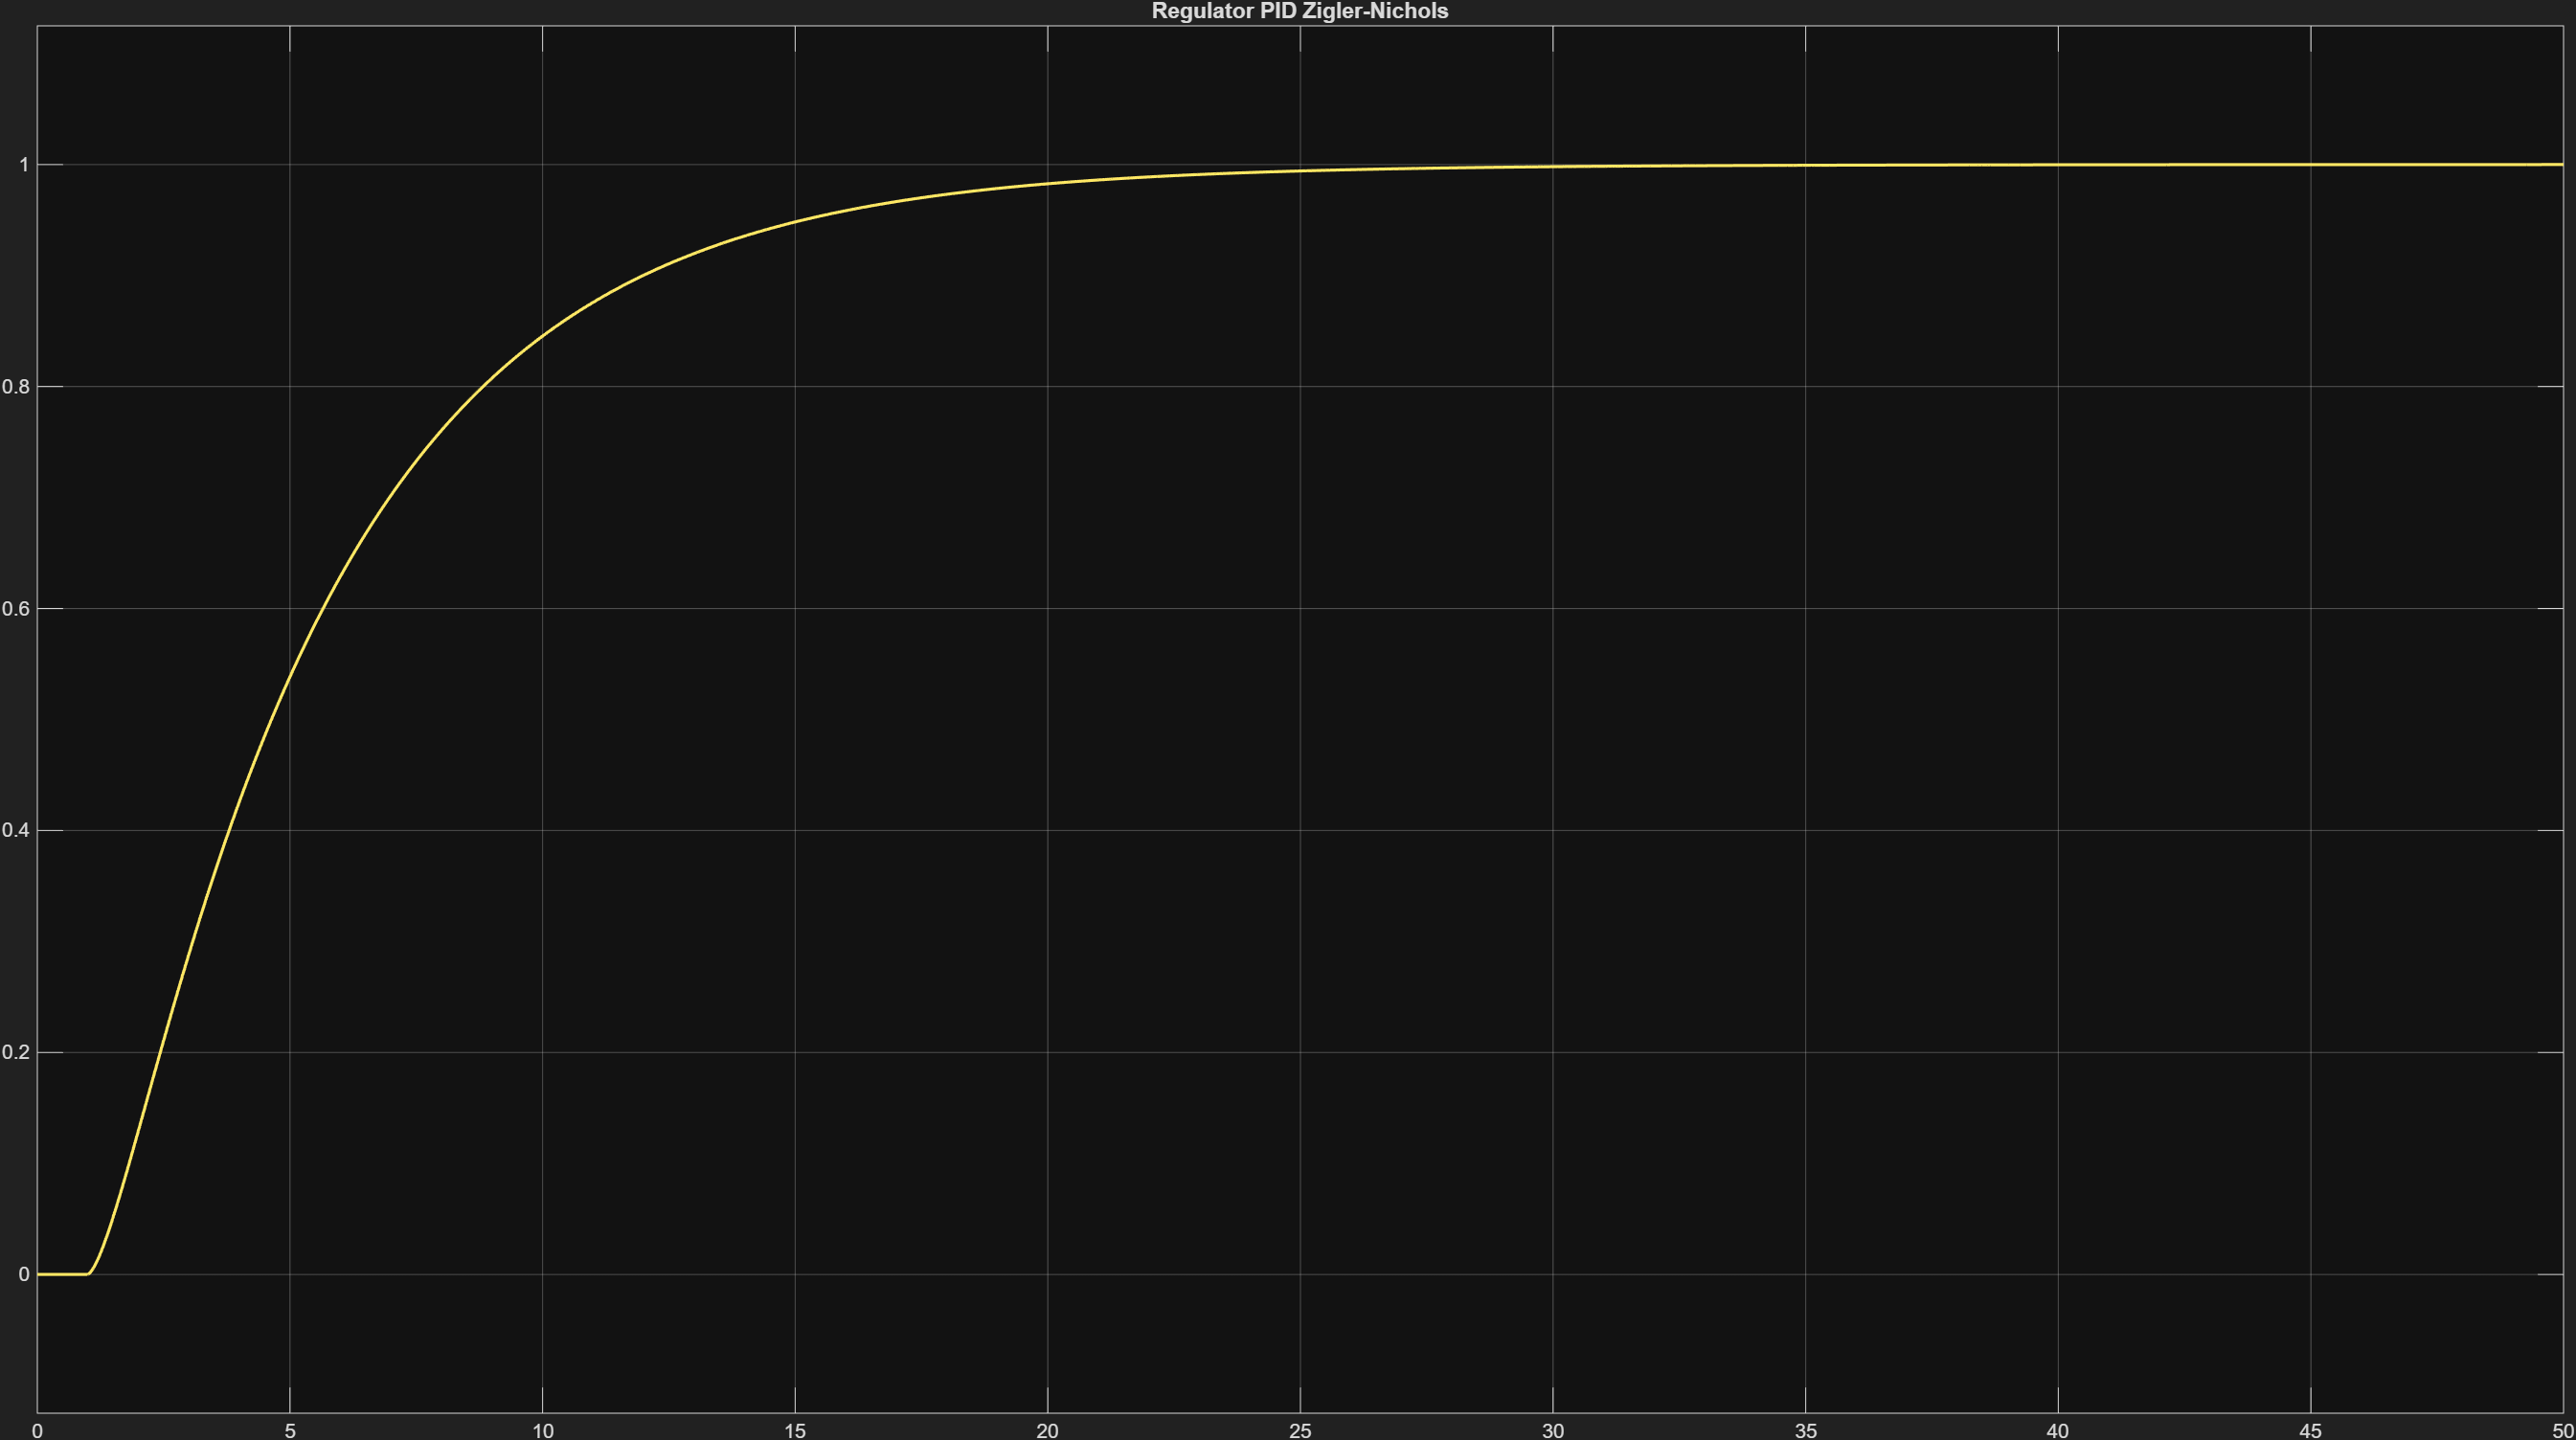
\includegraphics[width=0.7\linewidth]{../ScopePIDZN}
	\caption[]{Charakterystyka skokowa dla metody Zieglera-Nicholsa dla regulatora typu PID}
	\label{fig:PIDZN}
\end{figure}
\begin{figure}
	\centering
	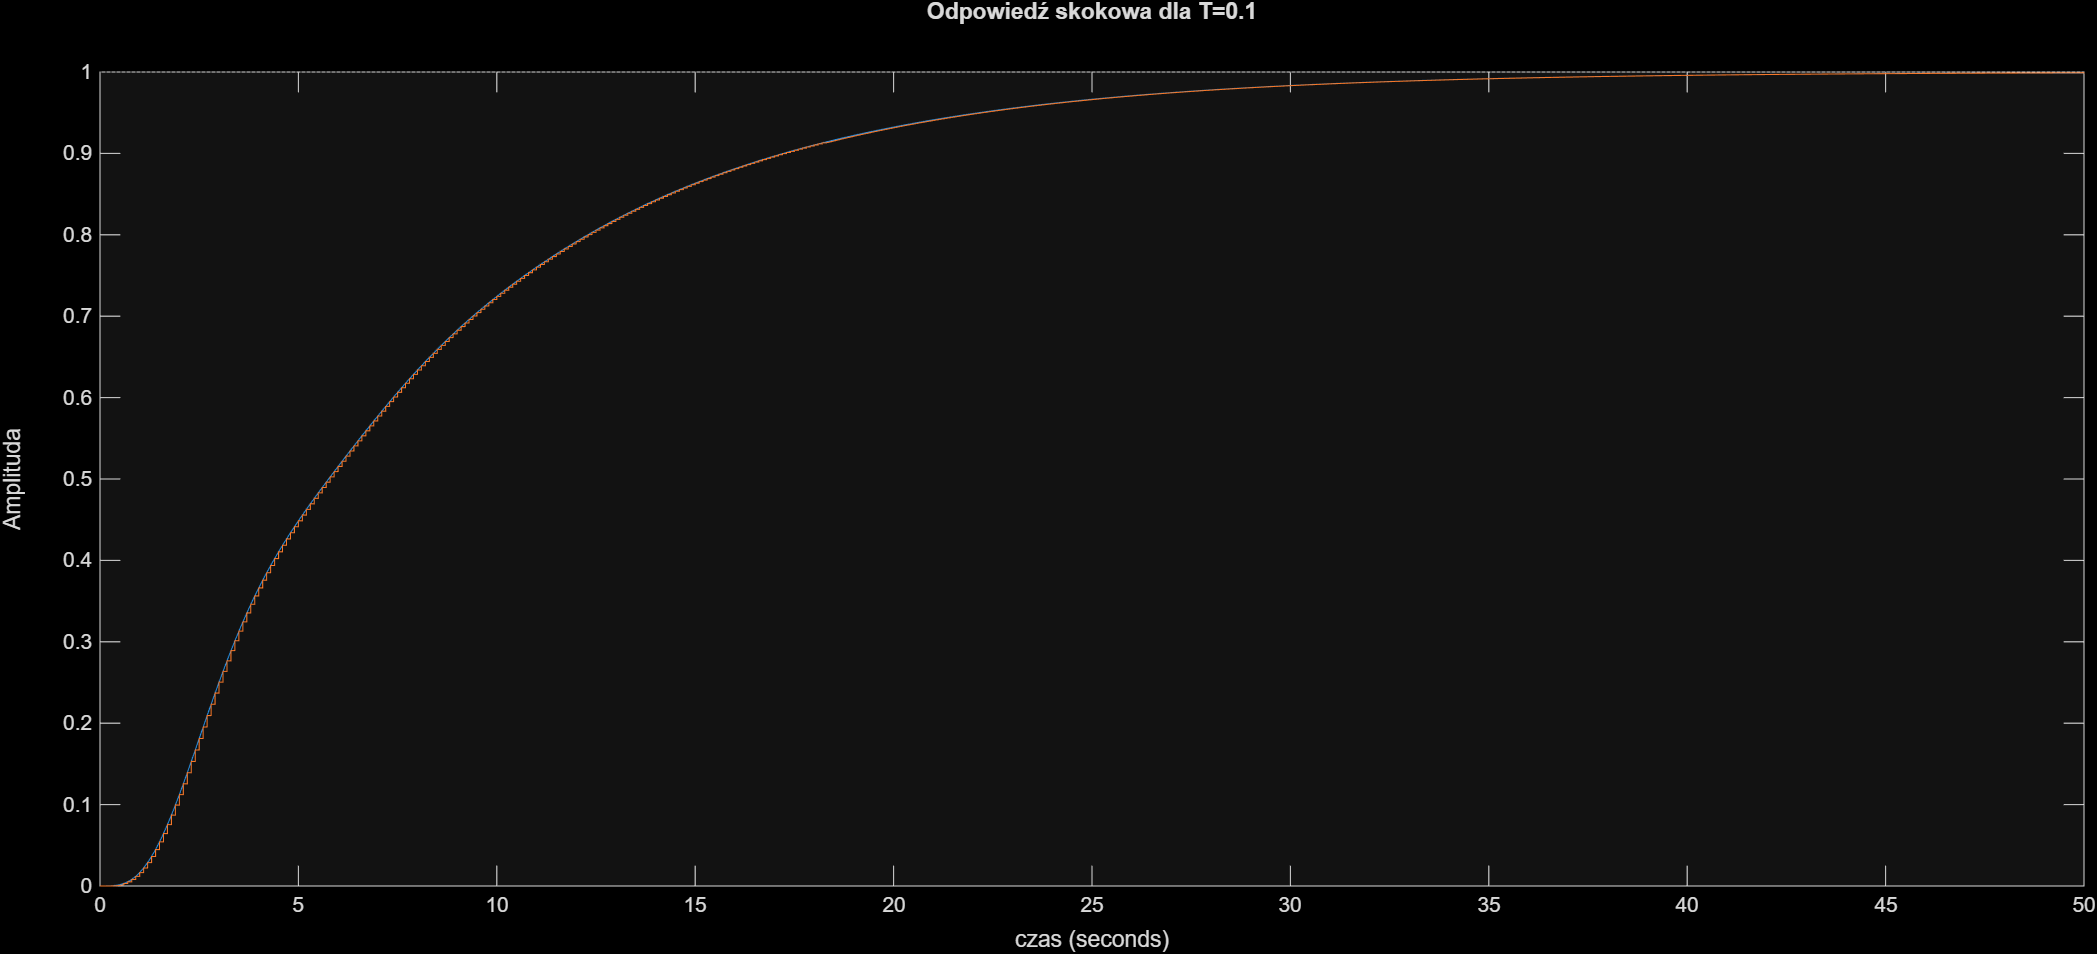
\includegraphics[width=0.7\linewidth]{../skok01}
	\caption{Odpowiedź skokowa obiektów dla T=0.1}
	\label{fig:skok01}
\end{figure}
\begin{figure}
	\centering
	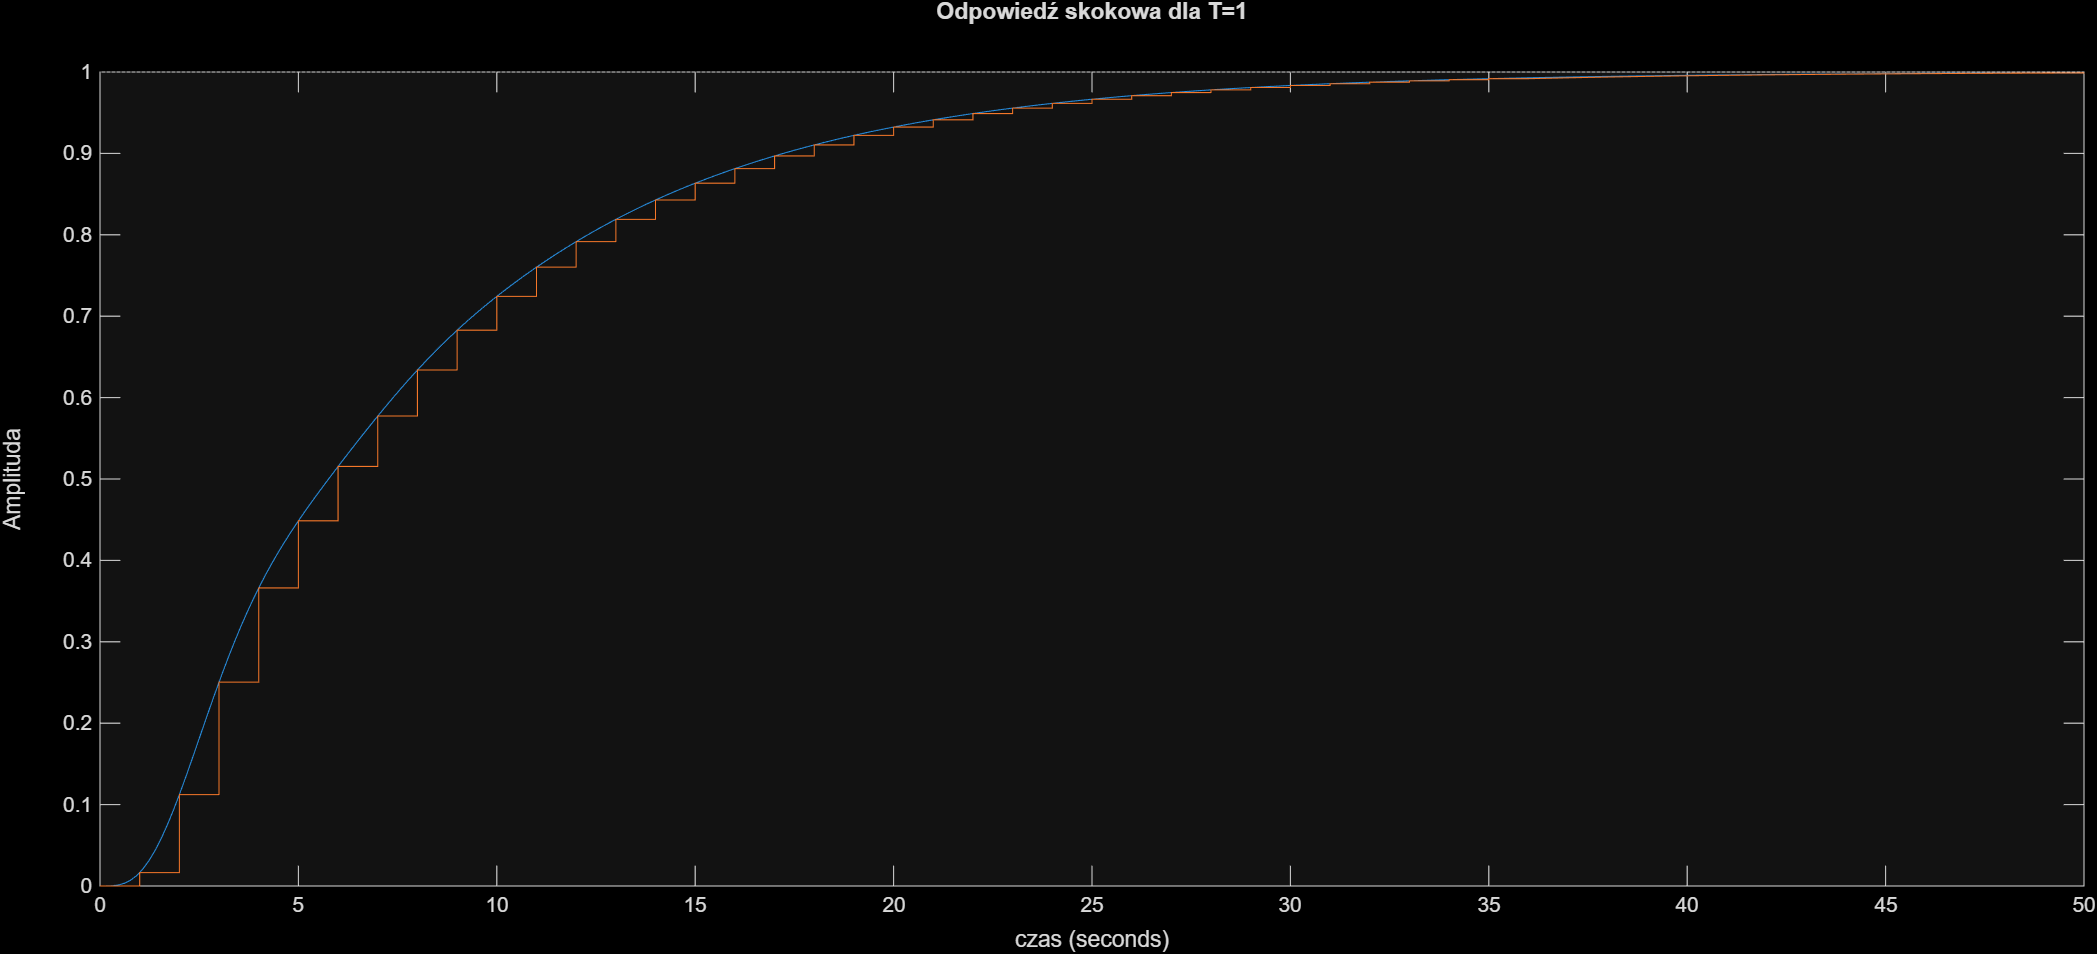
\includegraphics[width=0.7\linewidth]{../skok1}
	\caption{Odpowiedź skokowa obiektów dla T=1}
	\label{fig:skok1}
\end{figure}
\begin{figure}
	\centering
	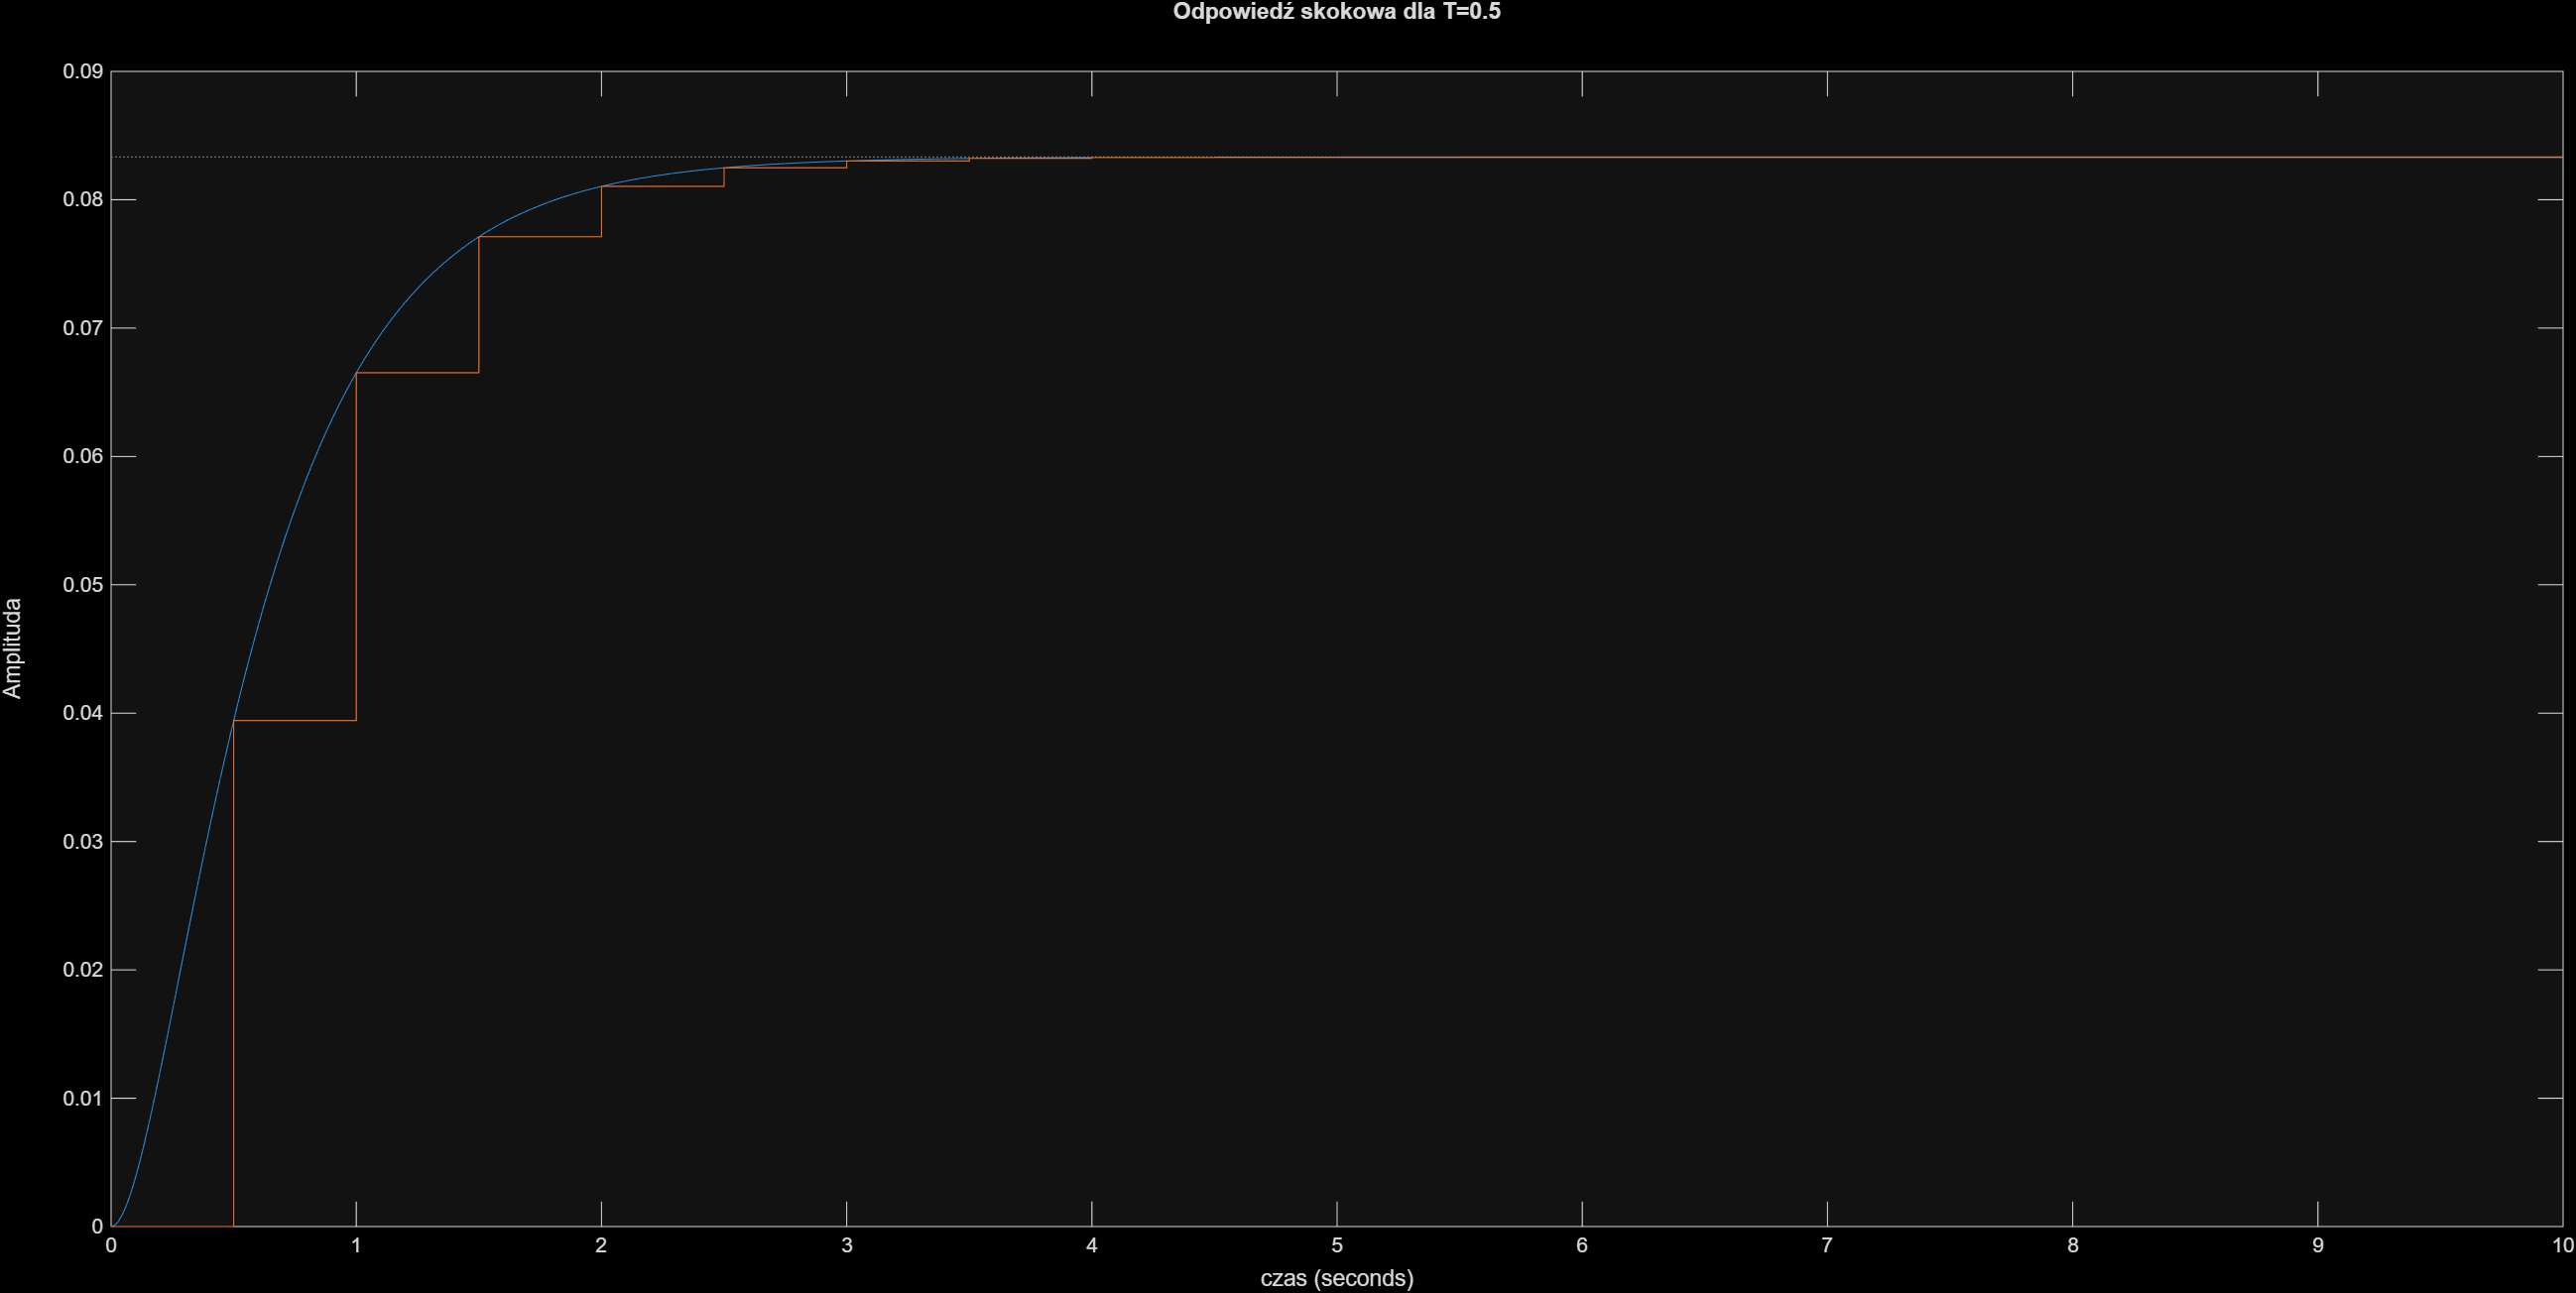
\includegraphics[width=0.7\linewidth]{../skok5}
	\caption{Odpowiedź skokowa obiektów dla T=5}
	\label{fig:skok5}
\end{figure}

\end{document}